%# -*- coding: utf-8-unix -*-
%%==================================================
%% thesis.tex
%%==================================================

% 双面打印
%\documentclass[doctor, openright, twoside]{sjtuthesis}
% \documentclass[bachelor, openany, oneside, submit]{sjtuthesis}
\documentclass[master, submit]{sjtuthesis}
% \documentclass[%
%   bachelor|master|doctor, % 必选项
%   fontset=fandol|windows|mac|ubuntu|adobe|founder, % 字体选项
%   oneside|twoside,        % 单面打印,双面打印(奇偶页交换页边距,默认)
%   openany|openright,      % 可以在奇数或者偶数页开新章|只在奇数页开新章(默认)
%   english,                % 启用英文模版
%   review,     % 盲审论文,隐去作者姓名、学号、导师姓名、致谢、发表论文和参与的项目
%   submit      % 定稿提交的论文,插入签名扫描版的原创性声明、授权声明 
% ]
% 逐个导入参考文献数据库
\addbibresource{bib/thesis.bib}
% \addbibresource{bib/chap2.bib}

%# -*- coding: utf-8-unix -*-
% !TEX program = xelatex
% !TEX root = ../thesis.tex
% !TEX encoding = UTF-8 Unicode
\title{基于声波的手写签名认证研究}
\author{丁峰}
\advisor{王东副教授}
% \coadvisor{某某教授}
\defenddate{2019年5月12日}
\school{上海交通大学}
\institute{电子信息与电气工程学院}
\studentnumber{117037910004}
\major{软件工程}
\keywords{手写签名认证, 智能手机, 声波, 非侵入}

\englishtitle{ Researches on Acoustic-based Handwritten Signature Verification }
\englishauthor{\textsc{Feng Ding}}
\englishadvisor{Associate Prof. \textsc{Dong Wang}}
% \englishcoadvisor{Prof. \textsc{Uom Uom}}
\englishschool{Shanghai Jiao Tong University}
\englishinstitute{\textsc{School of Electronic Information and Electrical Engineering} \\
  \textsc{Shanghai Jiao Tong University} \\
  \textsc{Shanghai, P.R.China}}
\englishmajor{Software Engineering}
\englishdate{May 12th, 2019}
\englishkeywords{Handwritten signature verification,  smartphone, acoustic signals, non-intrusive}

  % NOTE: the enclosed commands must be executed in preamble

\begin{document}

% 无编号内容:中英文论文封面、授权页
\maketitle

\makeatletter
\ifsjtu@submit\relax
  \includepdf{pdf/original.pdf}
  \cleardoublepage
  \includepdf{pdf/authorization.pdf}
  \cleardoublepage
\else
\ifsjtu@review\relax
% exclude the original claim and authorization
\else
  \makeDeclareOriginal
  \makeDeclareAuthorization
\fi
\fi
\makeatother

\frontmatter % 使用罗马数字对前言编号

% 摘要
%# -*- coding: utf-8-unix -*-
% !TEX program = xelatex
% !TEX root = ../thesis.tex
% !TEX encoding = UTF-8 Unicode
%%==================================================
%% abstract.tex for SJTU Master Thesis
%%==================================================

\begin{abstract}

手写签名作为一种生物特征,被广泛用于进行生物识别,并且具有相当长的应用历史。它被作为一种文件的授权方式已经有很长时间,因为它包含了个人独特的生物特征。在过去的时候,计算机技术还没普及大众,由于手写签名只需要一张纸和一只笔,使得授权操作变得很方便。在金融、法律、政府领域,手写签名也仍然是一种普遍的授权方式。然而,和人脸、指纹、虹膜、语音这些生物特征类似,手写签名可以被仿造。在银行业,一个仿造的签名能让一个非法的交易成功受理并通过,最后造成一笔巨大的损失。而且,签名仿造不单单发生在银行业,只要有用到手写签名认证的地方,都有可能遭遇仿造攻击,比如遗嘱签名的仿造。 当仿造者拿到真实签名的字迹后,可以花足够的时间去仿造这个签名,以至于仿造签名和真实签名非常相似,这给签名认证带来了巨大的挑战。

随着信息技术的兴起,目前为止很多自动签名认证系统已经被提出并且被应用到工业界中。与脸、虹膜等人体上的物理生物特征不同的是,手写签名会随着个体的身体和心理状态的变成而发生改变。 因此, 一个可行的签名认证系统需要对个体内的差异不敏感,对个体间的差异敏感。根据捕捉签名的方式的不同,现有的系统可以分成两类:离线签名认证系统和在线签名认证系统。离线签名认证系统扫描纸上的静态手写签名并分析,最后得出判别结果。相反,在线签名认证系统利用了笔的速度和压力的时间序列,而不是不是静态数据,执行认证操作。由于额外的时间维度上的信息,在线签名认证比离线签名认证通常可实现更高的精度。

本文实现了一种使用智能手机实现了一个非侵入式的不需要定制设备的手写签名认证系统 --- ASSV。虽然越来越多的用于签名认证的平板得到普及,但是一张纸盒一张笔用于签名依然非常常见。 相比于使用惯性传感器 (基于腕表),声波可以获得更细粒度的手的运动信息。声波信号普及率高,普通的智能手机便可发射和接收声波,可用于普世计算,近些年得到了众多研究者的关注。 本系统面向于这样的一个场景,用户使用普通的笔在普通的纸上签名,同时放在一旁的智能手机发射和接收人耳不可听的声波跟踪手的运动。
将声波应用到在线签名认证的过程中,本文主要做了以下几个方面的研究工作:

\begin{enumerate}[label=(\arabic*)]
    \item 据本文所知,这是第一个用智能手机发射和接收声波实现在线签名认证的系统。 本文实现了一个同时播放经过特定调制过的声波信号和接收声波信号的安卓应用,并在智能手机上高校执行预处理和特征提取的处理过程。 整个系统和用户低延迟交互。
    
    \item 使用声波的相位相关信息跟踪用户行为得到进一步研究。 本文提出了一种基于弦的方法去估计相位相关的信息,同时解决了直流问题。 使用数学方法证明该方法的可行性,以一种易于理解的方式呈现细节推理部分。 设计了特征提取和判别方法。
    
    \item 本文全面评估了ASSV系统。据结果显示,ASSV可以达到98.7\% 的 AUC (Area Under Curve) 和 5.5\%的 EER (Equal Error Rate), 且具有较低的延迟。 ASSV在交叉用户验证中也显示出了较好的性能。 当改变环境、时间、位置的情况,ASSV表现出良好的鲁棒性。更进一步,ASSV的安全性本文使用了重放攻击进行了测试。
\end{enumerate}


\end{abstract}
\begin{englishabstract}

As one kind of biological characteristics of people, handwritten signature has a long history of being used for biological identification. Handwritten signature has been regarded as one of main means of demonstrating the authenticity for paper-based
documents for a very long time because it contains the unique biological characteristics of an individual. In the past, handwritten signatures make authentication much easy as they only require a pen together with paper. Due to this, handwritten signature verification is commonly accepted as an authentication method in financial, legal, and administrative areas. However, similar to other biometric characteristics such as a face, fingerprint, iris and voice, handwritten signatures are also meeting the challenge of forgery. In the banking industry, a forged handwritten signature of payment can make the bank approve an illegal deal, which causes a large amount of loss. Moreover, such cases do not only occur in the financial area. Testamentary fraud is a new phenomenon, and forgery of signatures on a will brings the criminals a large amount of money. It is difficult for a person to recognize whether a signature is forged when the skilled forger has practiced forging this signature for a while.

With the rising of information technology, many handwritten signature verification systems up to now have been proposed and being used in the industry. Unlike the physiological characteristics (face, iris, etc.), signatures written in a period of time is affected by
the physical and emotional conditions of a subject. Therefore, a signature verification system is thought to be feasible only if the system is insensitive to intra-personal variability but sensitive to inter-personal variability.Existing systems can be categorized into two groups in terms of the method used to capture the signatures: off-line and on-line. In off-line verification, the static shapes of signatures are scanned and further analyzed. In contrast, on-line systems utilize the time series of speed and pressure of pens instead of static data to perform verification. Due to the additional temporal information, on-line approaches can achieve higher accuracy than off-line approaches.

This paper implements a non-intrusive handwritten signature verification system using a smartphone without special devices, ASSV. Although more and more digitizer devices have been employed, a pen together with paper is still common nowadays. Instead of inertial sensors, acoustic signals are exploited to get more fine-grained movement information of the hand non-intrusively. In addition, the applications of acoustic signals from smartphones have been researched in recent years. Hence, the system targets at the scenario where a user writes his signature on the normal paper with a normal pen while a smartphone transmitting and receiving inaudible acoustic signals is put aside to record the signal changes caused by the movements of both the hand and the pen. The main contributions of this paper are summarized as follows: 
\begin{enumerate}[label=(\arabic*)]
	\item To the best of our knowledge, this is the first work that implements handwritten signature verification only using the acoustic signals transmitted and received by smartphones. An android application is implemented to play the intended sound file and record the sound simultaneously. Preprocessing and feature extraction are implemented efficiently on the smartphone. The whole system interacts with users with a low latency.
	\item Tracking behaviors using the phase-related information of acoustic signals is studied. We propose a \mbox{chord-based} method to estimate the phase-related measurements resolving DC problems. Further, the feasibility of the method is proved mathematically and the detail of the proving process  is presented in an understandable form. The feature extraction and recognition methods are designed.
	\item We evaluate ASSV extensively. The results show that ASSV achieves an AUC of 98.7\% and an EER of 5.5\% with a low latency. ASSV also shows good performance in the cross-user usability test. And ASSV shows its robustness in the settings with varying environments, days and positions. Further, replay attack is applied to test its security.
\end{enumerate}

\end{englishabstract}



% 目录、插图目录、表格目录
\tableofcontents
\listoffigures
\addcontentsline{toc}{chapter}{\listfigurename}     % 将插图目录加入全文目录
\listoftables
\addcontentsline{toc}{chapter}{\listtablename}      % 将表格目录加入全文目录
\listofalgorithms
\addcontentsline{toc}{chapter}{\listalgorithmname}  % 将算法目录加入全文目录

%\include{tex/symbol} % 主要符号、缩略词对照表

\mainmatter % 使用阿拉伯数字对正文编号

% 正文内容
%# -*- coding: utf-8-unix -*-
% !TEX program = xelatex
% !TEX root = ../thesis.tex
% !TEX encoding = UTF-8 Unicode
%%==================================================
%% chapter01.tex for SJTU Master Thesis
%%==================================================

%\bibliographystyle{sjtu2}%[此处用于每章都生产参考文献]
\chapter{绪论}
\label{chap:intro}
\section{研究背景与意义}
本论文由上海市发展和改革委员战略新兴产业专项项目“基于物联网的当代艺术品电子商务公
共服务平台”、上海市经济和信息化委员会、上海市人力资源和社会保障局项目“上海市物联网技术
高技能人才培养基地RFID 应用实训设施设备环境资助”两个课题支撑。

\begin{figure}[!htp]
  \centering
  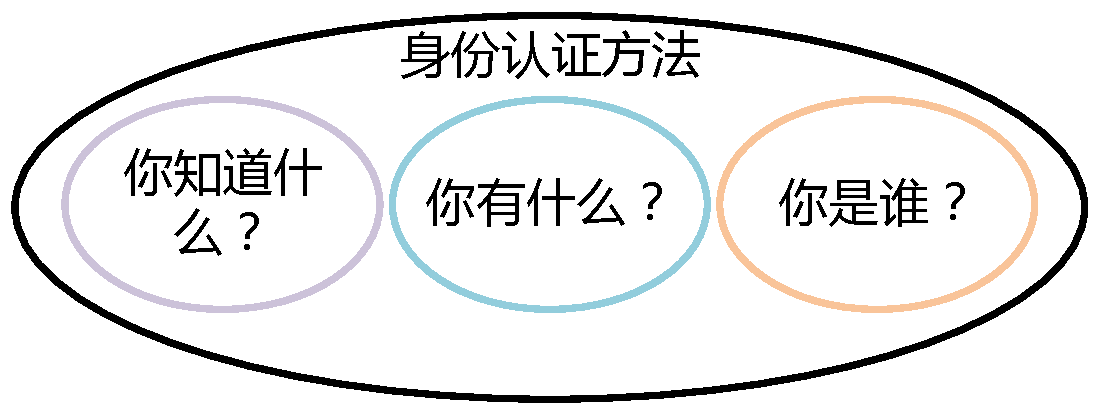
\includegraphics[width=0.7\textwidth]{figure/identification-method.pdf}
  \bicaption
    {身份认证方式}
    {Identification methods}
  \label{fig:identification-method}
\end{figure}
随着信息技术的兴起和广泛应用,许多应用需要用户首先进行登录操作,这其实就是身份识别方式,只有通过了通过身份认证的用户才会被系统认为是授权用户,用户才能访问到自己的隐私数据,比如地址信息、财务信息等。如图~\ref{fig:identification-method}所示,用户的身份方式可以为分为三种~\cite{Huang2011A}:
\begin{enumerate}[label=(\arabic*)]
    \item \textbf{根据用户知道的信息来证明身份。(你知道什么?)}日常生活中,我们以前最常用的是密码登录,这是一种依赖用户知道什么来识别是否为授权用户,但用户知道的密码被泄露,恶意用户输入相同的密码也会被系统识别为授权用户。
    \item \textbf{根据用户拥有的东西来证明身份。(你有什么?)}我们回家会使用钥匙开门,钥匙就是我们所拥有的东西,比起用户知道的信息,此处则体现为用户拥有的物理实体。
    \item \textbf{根据用户独一无二的身体特征证明身份。(你是谁?)} 随着智能手机的技术进步和普及,依靠智能手机上丰富的传感器配置,用户的认证方式也变多多样话起来,目前人脸和指纹识别已经被用于手机系统登录和移动支付。人脸~\cite{12717}、指纹~\cite{Andrew2005Handbook}、虹膜~\cite{Wildes1997Iris}等是人体上的固有特征,在随着时间变化上呈稳定状态,这样的认证方式比密码认证更加安全。 除此之外,个人独特的行为特征也可以被用于身份认证,比如:语音识别~\cite{Rashid2008Security}、唇语识别~\cite{Cetingul2006Discriminative}、步态识别~\cite{Boulgouris2005Gait}、手写签名识别~\cite{Plamondona1989Automatic}等。 
\end{enumerate}

手写签名作为个体的一种重要的行为特征,在金融、法律、政府等领域得到广泛应用,用于用户身份的识别,来识别一份文件的真实性。 相对应得,这种认证方式也会收到恶意用户的攻击,举个例子,攻击者可以仿造存款用户的签名去一张取款支票上签名从而去银行取款,会造成实际用户的财产损失,降低银行存款安全性,大则可引发金融灾难。 而在政府或军事领域,仿造签名会造成更加难以想象的结果,造成社会不公平和混乱。 因此,在这些签名进行授权的领域,签名的识别变得尤其重要。在很久以前甚至现在,签名的识别靠人工进行,签名验证者用户的历史签名在判断当前的签名是否为真实签名。这种方式,需要耗费昂贵的人力资源,且依赖于签名认证员的个人能力,容易造成错误。

信息技术将签名认证方式进行了自动化,自动签名认证系统得到研究和应用。 自动签名认证系统根据捕捉签名的方式不同,可以被分为两大类:离线签名认证系统和在线签名认证系统。 离线签名认证系统依靠签名图像的静态数据进行签名的比较来识别,而在线签名认证系统则依靠用户书写过程中记录下的时间序列数据(如书写速度、笔的压力等)来进行比较和识别。由于,外加的时间维度信息,通常在线签名认证系统的表现由于离线签名认证系统。

\begin{figure}[!htp]
  \centering
  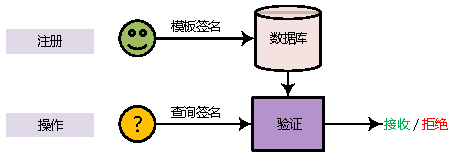
\includegraphics[width=0.7\textwidth]{figure/verification-work-flow.pdf}
  \bicaption
    {签名认证过程}
    {Signature verification architecture}
  \label{fig:signature-verification-architecture}
\end{figure}

无论是人工的签名识别还是自动签名认证系统,签名的识别的过程都符合图~\ref{fig:signature-verification-architecture}所示的这个签名认证过程。 在注册过程,用户需要收入多个他/她的签名给系统存入数据库作为模板签名;在操作过程,用户签下签名作为查询签名提交给系统,系统将这个查询签名和模板签名进行比较,判断查询签名是否为真实签名。

一个签名认证系统,识别任务的关键问题在于二方面:
\begin{enumerate*}[label=\itshape\alph*)\upshape]
    \item 需要能精准跟踪手写签名过程的行为信息。由于手写签名过程,笔记变化多样,而且运动幅度较小,对传感器的敏感度有较高要求。
    \item 用户体验和判别精度。用户体验体现在设备对用户的影响,比如是否需要特殊设备、是否需要用户佩戴设备等,还体现在模板签名数量。用户体验可能会和判别精度发生冲突,比如减少的模板签名数量会导致判别精度下降,复杂的设备则能更细粒度跟踪签名运动轨迹,有利于判别精度的提升。
\end{enumerate*}

开展自动手写签名认证的研究才能顺应用户对用户体验和财产安全提升上的诉求,将一部分人力资源从签名识别中解放出来,提高签名识别的准确率和稳定性,有利于维护金融和社会稳定。探索签名的捕捉方式,可以降低签名认证的成本,让签名认证系统在用户中快速普及。 目前国内外对手写签名认证的研究有很多基于开放数据集进行研究,存在一些问题,在普适性和用户体验上有待提高,所以本课题具有较好的研究意义和指导价值。

\section{国内外研究的现状}
如上文所述,手写签名认证研究的关键问题主要在两个方面,一是数据的来源问题,而是手写签名认证的建模问题。下面本节将从这两个方面对现有研究进行介绍。

(1) 数据来源问题的研究现状

在数据来源方面,现有的手写签名认证系统的研究主要依赖于惯性传感器、手写平板设备和扫描图像。其中前二者可用于实现在线签名认证系统,而离线签名认证系统则依赖于扫描图像的数据来源。

基于惯性传感器的方法~\cite{levy2018handwritten,griswold2019wearables,bunke2011online}利用穿戴在手上的惯性传感器 (速度计、陀螺仪等) 跟踪手部运动,提取个人签名时独特手部运动特征。这种方法,要求用户的穿戴的设备会给用户造成额外的困扰,设备穿戴的位置不宜固定,且会对结果造成较大影响。这里的惯性传感器设备包括:定制设备、腕表和装有惯性传感器的笔。

基于手写平板设备的方法~\cite{fischer2015robust,kholmatov2005identity,sae2013simple}利用手写笔或者手指在平板书写留下的动态轨迹来识别签名。这样的轨迹在静态轨迹基础上,还能获得书写时对平板压力和轨迹变化速度等时间序列,相比单单用静态图像可以大大提高判别精度。但是这样的设备需要一个手写平板,虽然我们可以利用上智能手机代替,但是这种方式限制了字迹不能写在平板上,而不能写在纸上这样我们生活最常见的场景。

基于扫描图像的方法~\cite{hafemann2017learning,hafemann2018fixed,ferrer2005offline,kalera2004offline}使用扫描仪扫描并切割出的签名图像,这种直接比较静态图像,与人工判别的方式在数据来源上有相似之处。由于没有写的过程,这种只比较写出结果的方法,无法判断出在字迹上看起来很相似仿造签名,尽管仿造者用较多的时间才仿造出了这个签名。但这种签名认证方式很有通用性和较好的用户体验,不会给用户签名过程造成干扰,用户可以依照平时的签名习惯来签名。

(2) 手写签名认证建模问题的研究现状

在手写签名认证建模方面,方法有多种多种,首先针对离线和在线签名认证系统需要采取不同的建模方法。在离线签名认证系统中,则能采用图像匹配的方法,比如人工神经网络(Artificial Neural Network, ANN)~\cite{chandra2016offline}、像素匹配 (Pixel Matching Technique, PMT)~\cite{bhattacharya2013offline}等。 在在线签名认证系统中,又可以分为两种:\textit{a)} 基于函数的方法,使用长短时记忆网络 (Long Short-Term Memory, LSTM)~\cite{hochreiter1997long}, 隐马尔科夫模型 (Hidden Markov Model, HMM)~\cite{rabiner1986introduction}, 动态时间规整 (Dynamic Time Warping, DTW)等这些函数型方法直接在时间序列上进行处理并识别;\textit{b)} 基于特征的方法,这种方法首先对时间序列从时域数据转化为频域数据,可以用到的变换方法有离散傅里叶变换 (Discrete Fourier Transform, DFT)、离散余弦变换 (Discrete Cosine Transform, DCT)~\cite{}等,在频域特征上进行特征选择从而实现数据的降维,在利用提取到的特征进行比较或者分类。匹配方法也可以使用DTW或者欧式距离,而分类方法可以使用一些机器学习方法~\cite{周志华2016机器学习},比如支持向量机 (Support Vector Machine, SVM)、随机森林 (Random Forest)、朴素贝叶斯 (Naive Bayes)等。这些很多方法都是在公开数据集上进行实现和评估的,当有新数据源时,我们需要设计新的合适的模型。而且,由于使用的是公开数据集,这些研究很少评估系统的鲁棒性,比如不同时间段对签名的影响。

\section{本文研究内容与创新点}
\subsection{研究内容与所做的工作}
在本文中,我们针对现有存在的主要问题着重研究设计一种非侵入式、鲁棒的、安全的、低延迟的在线手写签名认证方案,主要的研究内容和本文主要所做的工作如下:

(1) 手写签名认证数据源的研究

本文提出利用声波感知技术来跟踪手写签名时的运动手部和笔的运动状态,进而推断是否为本人签名。声波对我们来说不是陌生的信号,我们用声带发射声波,用耳膜接收声波,以此来实现对这个世界的感知。普通的智能手机上的扬声器和麦克风便能发射和接收声波,近年来,声波感知研究大量涌现,比如轨迹追踪~\cite{wang2016device,mao2016cat,yun2017strata}、呼吸检测~\cite{WangContactless,wang2018c}、手势识别\cite{ruan2016audiogest,gupta2012soundwave,aumi2013doplink,ling2018ultragesture}、成像\cite{mao2017aim}等。
假设声波信号的频率和传播速度分别是17000 Hz 和 346 m/s, 那么波长经计算为  $346/17000\approx0.02m$. 这么小的波长意味着声波的相位信息对周围物体的运动很敏感。本文采用声波的相关信息,利用计算弦的方法避开了求相位时去直流的问题,实现了微小动作的跟踪。


(2) 手写签名认证模型的研究

所有手写签名认证系统的大致框架前文已经有所提及,本文则针对声波的相位相关信息设计了合适的特征提取和用户独立的识别模型。手写签名动作所产生的影响在相位信号中体现为低频信号,而高频信号则是由环境或者硬件造成的噪声所产生。因此可以通过将时域数据转换到频域数据,然后提取低频系数的方法,将手写签名动作的信息提取出来。DFT是一种常见的获取频域数据的方法,但它的系数是2倍冗余的复数系数,所以我们采用DCT作为到频域数据的转换方法,并提取其前几个低频系数作为特征。当判别一个查询签名是否为真的时候,需要获取查询签名与模板签名之间的相似度,在此处,便是比较查询签名的特征与模板签名特征的之间的相似度。本文对多个模板签名的特征进行融合操作,获得几个固定数目的特征矩阵,查询签名的特征矩阵和这些矩阵作差获得相似矩阵。最后设计比传统分类器有更好表现的深度神经网络 (Deep Neural Network, DNN)\cite{Schmidhuber2015Deep} 作为一个二分类器,去分类相似矩阵。

(3) 基于声波的手写签名认证的系统实现和性能评估分析

本文针对所提出的基于声波的手写签名认证的方案,利用三星Galaxy S6智能手机设计并实现基于声波的手写签名认证系统,并且对其进行了全面的评估,包括准确性的度量、鲁棒性测试、安全性测试、微基准测试、性能测试等。准确性测试以 AUC (Area Under Curve) 和 EER (Equal Error Rate) 作为度量指标。在鲁棒性测试中,改变环境、距离、日期来对系统进行测试,观察准确性的变化。在安全性测试中,是模拟重放攻击,从而测试系统对此类攻击的抵抗能力。在微基准测试中,改变一些超参数,来观察系统的变化,以便设置较合适的超参数。在性能测试中,度量系统延迟,来判断系统是否具有良好的用户体验和是否对硬件要求过高。


\subsection{研究创新点}

本文主要有如下两个方面的创新点:
\begin{enumerate}[label=(\arabic*)]
    \item 本文第一次提出使用声波感知技术来实现一个在线签名认证系统,并基于一个三星Galaxy S6智能手机实现了一个非侵入式、用户友好、安全、低延迟、准确的在线签名认证系统。而且相比于之前的声波感知技术,在避免去直流的前提下,提取到了相位相关信息,用以跟踪手写签名时所产生的微小的动作。

    \item 本文针对新产生的信号,设计了特征提取方法和分类方法,并在进行了高效地实现。使用DCT提取信号中低频的有用的部分作为手写签名行为的特征,并使用深度学习进行分类,相比传统的分类方法获得了更好的表现。本文利用三星Galaxy S6智能手机设计并实现了基于声波的在线签名认证系统,全面评估了系统的性能。实验结果表明,本文提出的基于声波的在线签名认证系统的AUC可以达到98.7\%, EER可以达到5.5\%,并且是个安全、高效、鲁棒、低延迟的系统。
\end{enumerate}

\section{本文结构}

本文共分五章,每章的内容安排如下:

第一章为绪论,主要阐述了手写签名认证研究的背景意义、国内外相关技术的发展现状、本文的研究内容以及主要的创新之处。

第二章是手写签名认证相关技术的分析,首先分别从手写签名认证中的感知技术和手写签名认证中的建模方法两个方面对现有的研究进行了综述,然后分析总结了现有研究存在的问题。基于存在的问题,提出了本文的技术路线,最后介绍了本文中所涉及到的相关理论和技术。

第三章是基于声波的手写签名认证的关键技术研究,首先对要解决的问题进行了描述,然后提出一种基于声波的手写签名认证方案,该方案主要包含四个模块,对应了四种关键技术,然后依次对涉及到的声波相位相关信号感知技术、特征提取技术、相似性度量技术和深度学习模型进行了研究,详细描述了方案中各模块的设计思想和技术细节。

第四章首先对基于声波的手写签名认证方案进行了实验验证以及分析,手写描述了实验方法和采集的数据集,提出验证指标和用于对比的方案,之后实验验证本文方案的识别性能,最后探究影响识别性能的主要因素。

第五章基于本研究提出的基于声波的手写签名认证方案实现了一个基于安卓智能手机的手写签名认证系统,首先是对系统的用户需求进行分析,然后基于分析完成系统架构的设计,最后进行一系列评估实验来评估系统的性能效果。第六章是总结和展望,对本文的研究内容进行了总结,同时针对本文存在的不足,对未来的工作进行了一定的展望,并提出了系统可以改进的关键点。

\chapter{手写签名认证相关技术分析}
\label{chap:related-work}
目前手写签名认证的任务呈现普适性、便利性、模型用户无关的发展趋势,对实施技术的要求越来越高,在本章中我们将首先介绍手写签名认证研究综述,分析总结现有的研究存在的问题,然后针对存在的问题提出本文的技术路线,最后对本文涉及到的相关理论与技术进行介绍。
\section{手写签名认证研究综述}
手写签名认证研究所涉及到的技术领域比较广泛,如传感器技术、图像技术、通信技术、机器学习等等。应用这些技术需要解决的最核心的问题主要是两点,即“签名行为的数据怎么采集”和“采集到的数据怎么处理”。所以在手写签名认证的研究综述中,本文分别从手写签名认证中的感知技术和手写签名认证中的建模方法两方面进行综述。
\subsection{手写签名认证中的感知技术}
(1) 基于惯性传感器的手写签名认证
  
在手写签名的过程中,签名者通过手和笔的运动来留下签名字迹,运动过程中,手和笔的运动加速度和方向会发生变化,因此可以通过给手或者笔配备惯性传感器来实现对此运动过程的记录。常见的惯性传感器包括加速度计和陀螺仪,这两个惯性传感器均可产生三维的时间序列数据,分别记录物体线加速度和角运动,用于描述物体在三位空间中的运动状态。装配方式有两种:将惯性传感器装在手上,如智能腕表;将惯性传感器装在笔上。

\begin{figure}
  \centering
  \begin{minipage}[t]{0.3\textwidth}
    \centering
    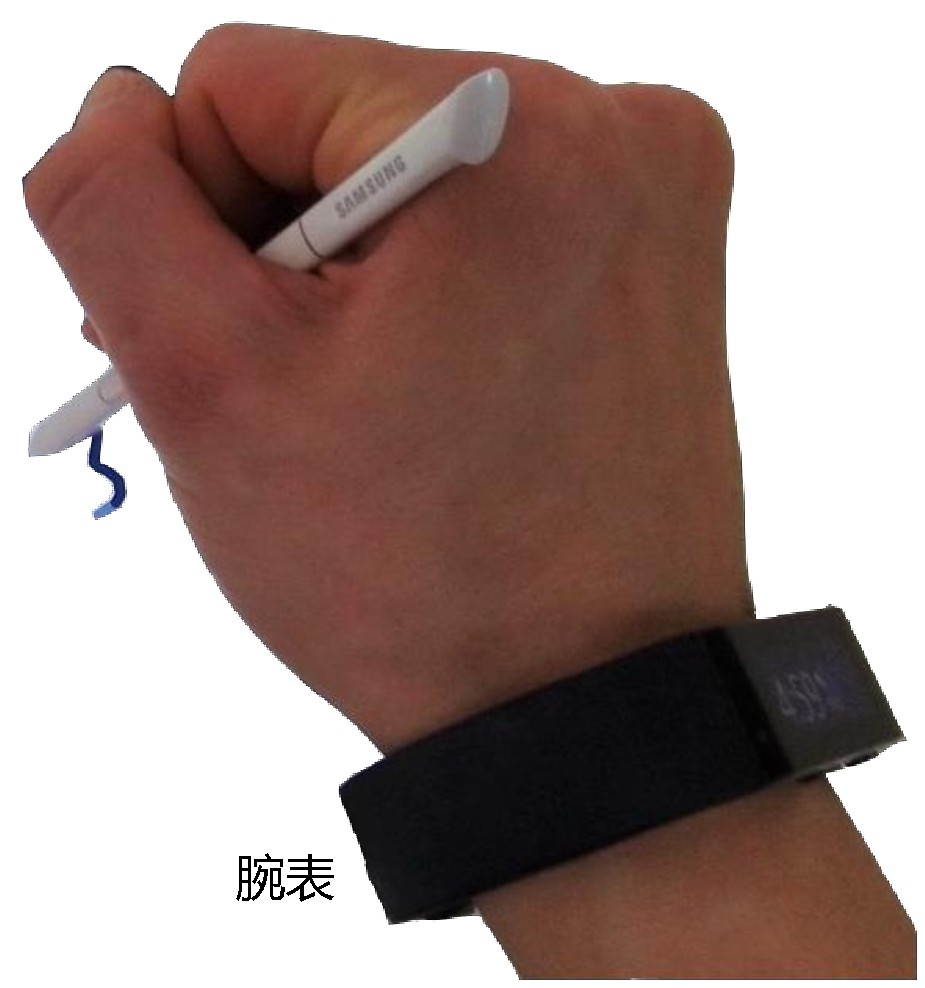
\includegraphics[width=\textwidth]{figure/smartwatch.pdf}
      \bicaption{用腕表上惯性传感器}
      {Using inertial sensors on swatches}
        \label{fig:smartwatch-inertial-sensor}
  \end{minipage}
  \centering
  \begin{minipage}[t]{0.49\textwidth}
    \centering
    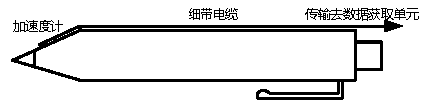
\includegraphics[width=\textwidth]{figure/acceleration-pen.pdf}
    \bicaption
    {用笔上的惯性传感器}
    {Using inertial sensors on pens}
    \label{fig:pen-inertial-sensor}
   \end{minipage}
\end{figure}
如图~\ref{fig:smartwatch-inertial-sensor}所示,基于腕表,Alona~\cite{Levy2018Handwritten}等人提出一种可穿戴的手写签名认证系统,它使用一个戴在签名手上的智能腕表上的惯性传感器和加速度计实现对签名动作的记录,虽然腕表目前的普及率还选不如智能手机,但腕表仍在受到大众的欢迎,所以这种方法具有普适性。Isaac\cite{8698222}等人使用腕表是实现了在多个场景下的手写身份识别,并对多种不同强度的攻击方式进行评估。使用如图~\ref{fig:pen-inertial-sensor}所示,基于笔上的加速度计,Bunke~\cite{Bunke2015Online}等人在普通笔的笔尖附近贴上了一个带线的加速度计,通过细带电缆将加速度时间序列传输到电脑端,依此分析签名动作。

(2) 基于扫描图像的的手写签名认证
\begin{table}[!hpb]
  \centering
  \bicaption
    {真实签名与仿造签名图像}
    {Genuine and forged signatures}
  \label{tab:signatures-images}
  \begin{tabular}{|c|m{0.2\textwidth}|m{0.2\textwidth}|m{0.2\textwidth}|} \toprule 
    类型 & 真实签名 & 熟练仿造签名 & 不熟练仿造签名\\ \midrule
   简单& 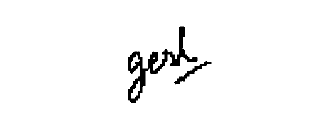
\includegraphics[width=0.2\textwidth]{figure/signature-1.png}&
\includegraphics[width=0.2\textwidth]{figure/signature-2.png}&
\includegraphics[width=0.2\textwidth]{figure/signature-3.png} \\ \midrule
    草书&
\includegraphics[width=0.2\textwidth]{figure/signature-4.png}&
\includegraphics[width=0.2\textwidth]{figure/signature-5.png}&
\includegraphics[width=0.2\textwidth]{figure/signature-6.png} \\ \midrule
    图形&
\includegraphics[width=0.2\textwidth]{figure/signature-7.png}&
\includegraphics[width=0.2\textwidth]{figure/signature-8.png}&
\includegraphics[width=0.2\textwidth]{figure/signature-9.png} \\ 
        \bottomrule
  \end{tabular}
\end{table}

如图~\ref{tab:signatures-images}所示,在图像上,签名通常可以被分为三类~\cite{Hanmandlu2005Off}:简单的、草书的、图形的签名。简单的签名便是平时的普通签名;草书签名是写的过程有比划连在一起的签名;图形的签名则是用草书方式描述几何模式的签名。从图像上真实签名、熟练仿造签名、不熟练仿造签名之间有很大相似之处,但是细看不同之处也有很多。离线签名认证利用这些从纸上扫描出来的图像进行识别。

Madasu~\cite{Hanmandlu2005Off}等让签名者使用黑笔在白纸上签名,之后使用扫描仪以200 dpi的分辨率扫描获得图像,并经过50\%的重采样将像素点数量减少到原来的一半。40个志愿参与数据集构建,每个志愿者提供15个真实签名和15个仿造签名,总共2400个签名图像。Subhash~\cite{chandra2016offline}等人邀请了18个志愿者,每个志愿者提供15个真实签名和15个仿造签名,总共540个尺寸为$850\times360px$的签名图像。除了自己手机签名数据集外,目前公开的签名图像数据集有:MCYT\footnote{http://atvs.ii.uam.es/atvs/mcyt75so.html}、CEDAR\footnote{https://cedar.buffalo.edu/Databases/CDROM1/}、Brazilian PUC-PR~\cite{freitas2008brazilian}. 签名的公开数据库文字上以英文居多,Brazilian PUC-PR则提供巴西葡萄牙语的签名数据。采集签名的方式,最传统的可以直接让志愿者写在纸上,然后扫描,这种方式较为费力。而最近,可以让签名者将签名写在平板上,仅仅使用静态轨迹数据就可以作为离线签名的数据集,同时兼顾离线签名认证研究和在线签名认证研究对数据集的需求。

(3) 基于手写平板设备的手写签名认证

\begin{figure}[!htp]
  \centering
  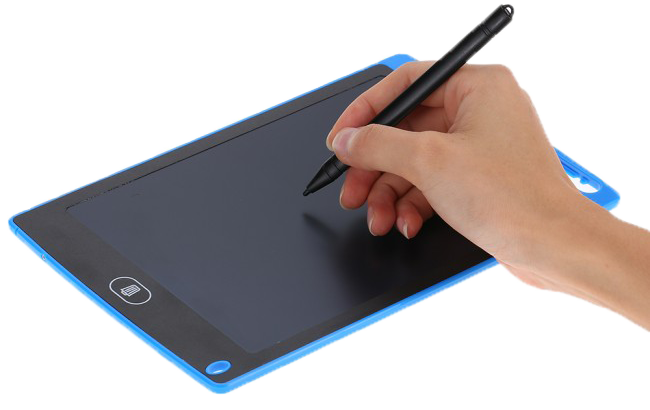
\includegraphics[width=0.5\textwidth]{figure/tablet.png}
  \bicaption
    {在平板上签名}
    {Signing on a tablet}
  \label{fig:signing-tablet}
\end{figure}
如图~\ref{fig:signing-tablet}所示,签名使用使用手写笔在平板上签名,由平板记录签名轨迹,手写屏除了记录轨迹还能记录压力值,如果使用智能笔则还能记录笔的倾斜角,因此时间序列数据可以包括:采样点的二位坐标、笔尖压力值、笔的水平偏角和垂直偏角。Alona~\cite{Levy2018Handwritten}等人在用腕表上惯性传感器跟踪签名动作时候,同时用手写记录签名轨迹,将平板上轨迹数据除了可以提给仿造者提供仿造学习材料,还可以用于和两个经典系统~\cite{fischer2015robust,kholmatov2005identity}做对比实验。目前,可用于在线签名认证研究的公开数据集有:MCYT-100\footnote{http://atvs.ii.uam.es/atvs/mcyt100s.html}、SUSIG~\cite{kholmatov2006sigsa}、SVC2004~\cite{10.1007/978-3-540-25948-0_3}、SCUT-MMSIG~\cite{10.1007/978-3-319-69923-3_78}等。

MCYT-100是MCYT数据库的一个子集,包含100个签名者的数据,每个签名者有25个真实签名和25个仿造签名,总共5000个签名样本。至于SUSIG数据库,Kholmatov~\cite{kholmatov2006sigsa}等人使用一个分辨率为300 dpi、具有128层垂直压力感知、100 Hz采样率的压力感知触摸平板,邀请110位志愿者参与真实签名的收集,其中包括年龄在21岁到52岁之间的29位女性和81位男性,每个位志愿者分两个时间段提供20个真实签名,而仿造签名由仿造者观看签名过程并联系后为每个真实签名者提供5个仿造签名,他们同时用实验结果签名是一个复杂度取决于签名者的生物特征。SV2004是2004年香港科技大学举办在线认证比赛提供的数据库,针对比赛中的两个任务,该数据库提供两个数据集,每个数据集都包含100个签名集合,每个签名集合包含20真实签名和20熟练仿造签名,不同是其中一个数据集只包含坐标时间序列,而另外数据集则还包含笔的方向和压力,两个数据集前40个集合完全不同,而后60个集合仅仅是笔的方向和压力不同。比赛中,成绩最好的第一个任务EER=2.84\%,第二个任务EER=2.89\%。SVC2004包含中文签名和英文签名,SCUT-MMSIG则是由华南理工大学采集的纯中文签名,所以如果做针对中文签名认证研究的研究者可以考虑这两个签名数据作为评估数据集。

此领域的研究者基于公开数据集做了很多工作。算法~\cite{kholmatov2005identity}提出SVC2004是的冠军提出。2015年提出的一个算法~\cite{fischer2015robust}在两个数据集上进行了评估,在MCYT数据集上使用5个模板签名时在随机仿造(random forger)和熟练仿造(skilled forger)情况下的EER分别为1.06\%和3.94\%,在SUSIG数据集使用5个模板签名时在随机仿造和熟练仿造情况下的EER分别为1.34\%和3.09\%。

\subsection{手写签名认证中的建模方法}

已经有很多文章对签名认证研究进行了综叙,如80年代的Rejean~\cite{plamondon1989automatic}等人的综叙,那时研究者开始用人工神经网络实现签名认证,还,有90年代的Franck~\cite{leclerc1994automatic}和2000年代的Donato等人~\cite{impedovo2008automatic}的综述,在2012年Donate等人对之前的综述进行了补充~\cite{impedovo2012handwritten}。近期,Luiz G.~\cite{hafemann2017offline}等人对离线签名认证进行了综述,并加入基于深度学习的相关研究内容。Prathiba~\cite{prathiba2014online}等人对在线签名认证进行了综述。

Kai~\cite{huang1997off}等人提取了签名图像的多种粒度的局部对比的几何特征,为每个力度的特征使用一个适配的多层感知机,多个感知机的输出作为一个决策感知机的输入,决策感知机用于输出最后二分类的结果,在一个超过3000个样本的数据库中达到90\%的分类准确率。为所有用户而训练的模型称为写者独立模型(writer-independent model, WI model),而需要为每个用户训练一个的模型称为写着依赖模型(writer-dependent model, WD model)。有些系统会使用熟练仿造签名进行用户独立模型的训练~\cite{rivard2013multi,eskander2013hybrid},而有些系统使用熟练仿造签名进行用户独立模型训练~\cite{yilmaz2016score,rantzsch2016signature,hafemann2017learning},再用另外一个分开的数据集进行测试。有些系统混合使用用户独立模型和用户依赖模型,使用用户独立模型用于特征提取,利用提取到的特征为每个用户训练一个小型的用户依赖模型,综合了两种模型的优点。随着深度学习在图像领域的广泛应用,现在可以用DNN直接从图像中学习得到特征。Hafemann~\cite{hafemann2016writer}等人使用一个卷积神经网络(Convolutional Neural Network, CNN)作为特征提取器,在用SVM为每个用户训练一个用户依赖模型,之后进步提出了多任务的卷积神经网络框架~\cite{hafemann2017learning},可同时提取到区分签名真实性和用户间差异的特征。

来自签名的动态特征提供提供了某个时间的比划数目和顺序,速度,笔的压力等相关信息,可以提高签名变得更加具有唯一性。 Alisher~\cite{kholmatov2005identity}等人的在线签名认证系统将签名的识别视为一个二分类的模式识别问题。DTW被用于建立给定签名的合法性:给定一个签名与被申明用户的参考签名计算DTW距离,计算出与最近、最远、模板参考签名的DTW距离,生成3维的特征向量用于后续的分类。在使用熟练仿造者的测试用,EER达到2.8\%。S.A. Daramolo~\cite{daramola2010efficient}等人为了建立签名的特征序列之间的一致关系,DTW被用于训练和分类。Alona~\cite{levy2018handwritten}等人结合使用DCT和DTW,得到一个特征向量,最后输入到一个用户独立的二分类进行判别。HMM被证明可以有效用于签名认证,应为它可以高度适应个体间差异。Mohammad M. Shafli 和 Hamid R. Rabiee~\cite{shafiei2003new}介绍了使用变长分段和HMM实现的在线签名认证系统,实现了错误接受率(False Accept Rate, FAR)和错误拒绝率(False Reject Rate)分别为4\%和12\%的性能。Syed Khaleel Ahmed~\cite{ahmed2009automatic}等人设计的签名认证系统由4个模块组成,分别是特征提取模块、参考模块、样本模块、智能决策模块。特征提取模块用于捕捉二位坐标和笔的压力的时间序列。参考模块用于存储训练数据。样本模块包含用于验证的数据。智能决策模块则是一个自组织映射神经网络,用于对数据进行聚类,将高维数据映射为1或2维数据。%Alona~\cite{levy2018handwritten}等人使用DCT对惯性传感器的数据转换去前几位低频系数,减少了数据量,将查询签名的DCT系数和模板签名的低频系数求DTW距离并去最小值,得到一个特征向量,最后输入到一个用户独立的二分类进行判别。

\section{现有研究存在的问题}
根据上文对于手写签名认证的研究综述,现分别从手写签名认证中的感知技术和建模技术这两方面对现有研究存在的问题进行分析总结。

(1) 手写签名认证的感知技术中存在的问题

目前,通常采用的手写签名认证中的感知技术方案主要有三种——基于惯性传感器、基于扫描图像、基于手写平板设备的解决方案。其中,基于惯性传感器的主要问题是,需要用户或者笔上佩戴惯性传感器,会给用户带来不便利性:如果是笔上安装惯性传感器,则要求定制的笔,不便于推广;如果是要求用户佩戴腕表之类的设备,则该设备必须在用户写字的手上,在可穿戴设备还没大量普及的前提下该要求过于苛刻,而且腕表在手上的位置变化也会提高判别的错误率。基于扫描图像的方法,比较符合用户的习惯,但是由于动态特征的缺失,熟练的仿造者可以话足够的时间去仿造他们的签名已达到在静态形状上尽可能像,这给离线签名认证系统带来了巨大的挑战。基于手写平板设备的方法,需要一个可以手写平板,如果用手指写则不符合用户平时的签名习惯,如果也是用笔在平板上写并且给予书写轨迹的反馈,还是需要特殊的设备,提高了普及化的难度。

(2) 手写签名认证的建模技术中存在的问题

DTW是一种非常经典用于计算两个不同长度的序列距离的算法,其在模式识别中的应用十分广泛。然而,DTW技术具有两个明显的缺点:(1)计算开销大,需要更多时间;(2)对仿造签名进行规整使得验证更加困难。而且HMM模型是无记忆性的,它的当前状态只与其前一个状态有关,无法利用更多复杂信息。使用深度学习进行用户无关的模型训练会引发巨大的训练开销,而且越是复杂的网络要求有足够大的数据集防止其过拟合。目前的系统大多在公开数据集进行测试,过于追求精度的提升,很少有度量在识别时间上的开销,因此复杂的方法在时间中不一定可行。

\section{本文的技术路线}
\begin{figure}[!htp]
  \centering
  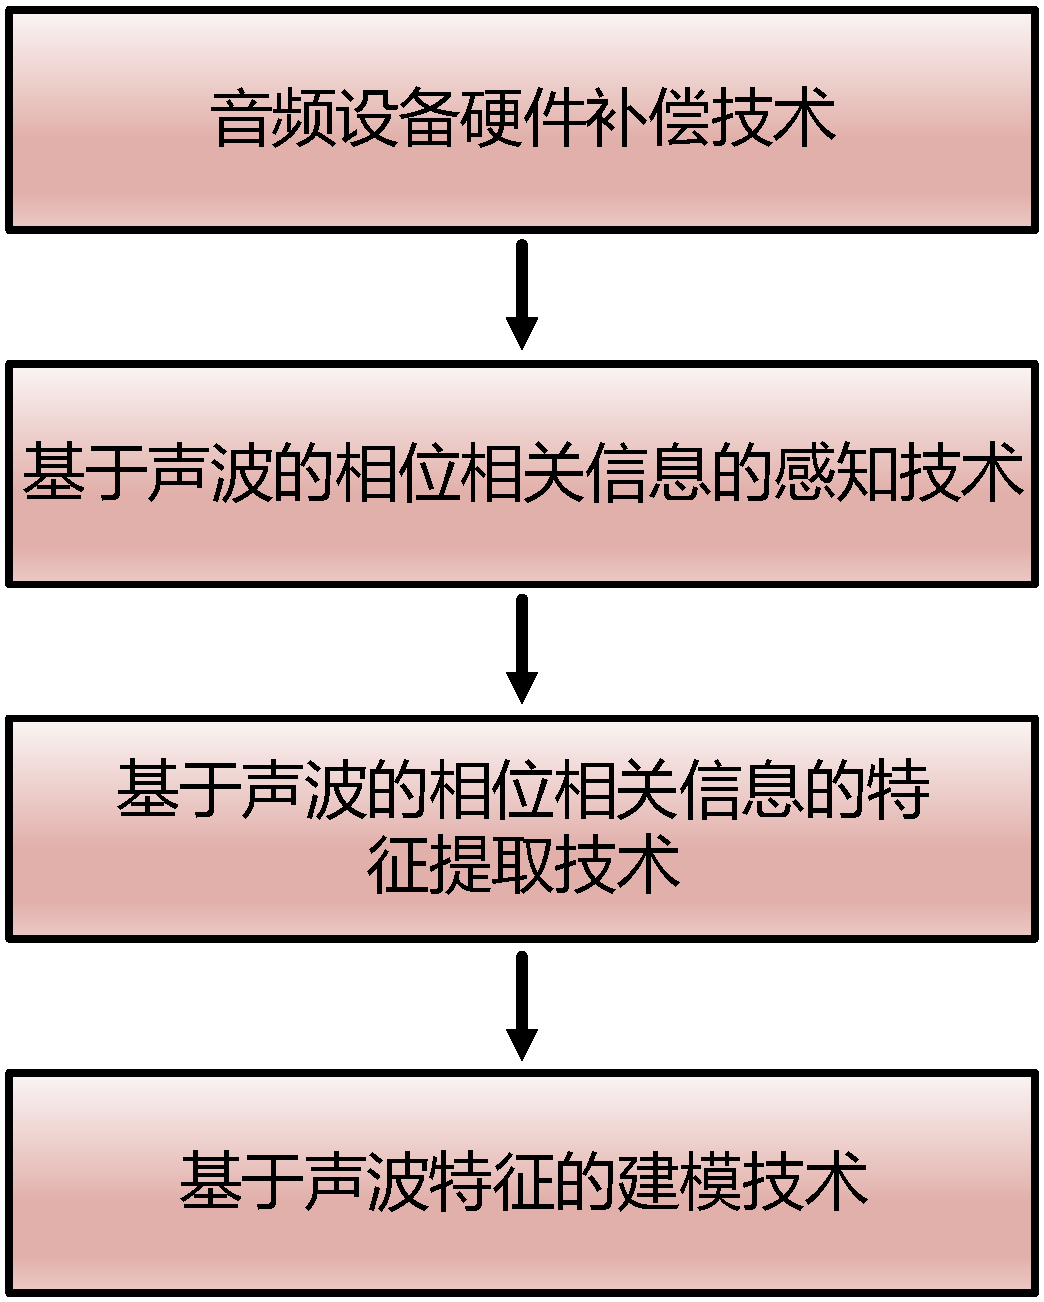
\includegraphics[width=0.4\textwidth]{figure/technique-road.pdf}
  \bicaption
    {本文的技术路线}
    {The technology roadmap}
  \label{fig:technology-roadmap}
\end{figure}
本文通过深入分析现有研究,针对目前手写签名认证中的感知技术和手写签名认证中的建模方法的研究中存在的问题,提出了本文的技术路线。技术路线如图~\ref{fig:technology-roadmap}所示,其中主要分为具有递进关系的四种技术研究,分别是音频设备硬件补偿技术、基于声波的相位相关信息的感知技术、基于声波的相位相关信息的特征提取技术、基于声波特征的建模技术。其中的箭头表示了这几种技术步骤之间的依赖关系,下面将分别介绍这四种技术。

(1) 音频设备硬件补偿技术

本文的数据采集和原型系统实现基于智能手机上的音频设备。然而,智能手机上的音频设备主要用于娱乐、通信、降噪等,其主要设计用途并不包括声波感知,因此当时利用智能手机发送高频的声波信号(17 kHz以上),尤其是同时发送多个高频声波信号时,每个频率说声波实际发送能量差异可能会很大。本文针对智能手机上的音频设备的硬件不足,进行了硬件补偿,以便目标频率声波的发射能量不至于太小。

(2) 基于声波的相位相关信息的感知技术

从麦克风设备中获得是一个原始的音频数据,其中包括了人交谈的声音、环境噪音等可听见和不可听见的声音。这些可见的声波信号并不是本文所需要的,我们需要对原始的接收信号进行下转换以后获得两个经降采样的正交信号,这两个正交信号可用于计算相位。相位信息声波的传播路径长度成直接相关,因此环境中一些周期性运动,比如笔记本散热器叶片的转动,会对相位信息产生影响。因此,需要对两个正交信号进行去噪,然后提取相位相关的信息。

(3) 基于声波的相位相关信息的特征提取技术

声波的相位信息和声波传播路径直接相关,签名时手的运动,引起声波传播路径长度的变化,从而导致相位的波动。而手的运动对相位的影响呈现为低频信号,高频信号则为噪声。本文使用DCT将相位相关信号从时域转换到频域,取低频系数作为特征提取和选择的结果。

(4) 基于声波特征的建模技术

本文认为签名真确性的判别是个二分类问题。对一个用户,在收集模板签名之后,根据这些所有的模板签名的特征矩阵,计算出三个(最小值、最大值、平均值)用于参与和查询签名比较的矩阵,和查询签名的特征矩阵通过作差得出其余模板的距离矩阵。本文设计一个多层CNN模型,以距离矩阵作为输入,进行二分类。

\section{相关理论与技术简介}

\subsection{智能手机音频设备的位置和配置}
\begin{figure}[!htp]
  \centering
  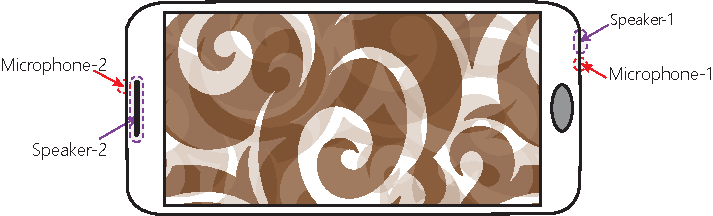
\includegraphics[width=0.7\textwidth]{figure/smartphone.pdf}
  \bicaption
    {智能手机上的音频设备}
    {Audio devices on smartphones}
  \label{fig:audio-device-smartphone}
\end{figure}

三星Galaxy S6是三星公司在2015年5月推出的一款智能手机,是本文原型系统ASSV使用的智能手机,因此以此为例进行说明。如图~\ref{fig:audio-device-smartphone}所示,该智能手机搭载了2个扬声器和2个麦克风:
\begin{enumerate*}[label=\alph*)]
    \item 一个降噪麦克风(Microphone-2)位于机身的上壁,对高频信号较为敏感,且原来用户打电话的时的发生点,可以用于记录背景噪声;
    \item 一个主麦克风(Microphone-1)位于机身的下壁,对人声比较敏感(通常低于8 kHz),用于记录通话语音;
    \item 一个通话扬声器(Speaker-2)位于屏幕上部,用于通话是对准耳朵;
    \item 一个主扬声器(Speaker-1)位于机身的下壁,位于主麦克风的旁边。
\end{enumerate*}

\begin{table}[!hpb]
  \centering
  \bicaption{三星Galaxy S6的硬件配置}{Hardware settings of Samsung Galaxy S6}
  \label{tab:smartphone-hardware-setting}
  \resizebox{\textwidth}{!}{
\begin{tabular}{|l|l|l|}
\hline
\multirow{2}{*}{Body}     & Dimensions  & 143.4 x 70.5 x 6.8 mm (5.65 x 2.78 x 0.27 in)                          \\ \cline{2-3} 
                          & Weight      & 138 g (4.87 oz)                                                                            \\ \hline
\multirow{4}{*}{Platform} & OS          & Android 5.0.2 (Lollipop), upgradable to Android 8.0 (Oreo); TouchWiz UI \\ \cline{2-3} 
                          & Chipset     & Exynos 7420 Octa (14 nm)                                                \\ \cline{2-3} 
                          & CPU         & Octa-core (4x2.1 GHz Cortex-A57 \& 4x1.5 GHz Cortex-A53)                \\ \cline{2-3} 
                          & GPU         & Mali-T760MP8                                                            \\ \hline
\multirow{2}{*}{MEMORY}   & Card slot   & No                                                                      \\ \cline{2-3} 
                          & Internal    & 32/64/128 GB, 3 GB RAM                                                  \\ \hline
\multirow{4}{*}{Sound}    & Loudspeaker & Yes                                                                     \\ \cline{2-3} 
                          & 3.5mm jack  & Yes                                                                     \\ \cline{2-3} 
                          &             & 24-bit/192kHz audio                                                     \\ \cline{2-3} 
                          &             & Active noise cancellation with dedicated mic                            \\ \hline
\multirow{5}{*}{Battery}  &             & Non-removable Li-Ion 2550 mAh battery                                   \\ \cline{2-3} 
                          & Charging    & Fast battery charging 15W                                               \\ \cline{2-3} 
                          &             & Qi/PMA wireless charging (market dependent)                             \\ \cline{2-3} 
                          & Talk Time   & Up to 17 h (3G)                                                         \\ \cline{2-3} 
                          & Music play  & Up to 49 h                                                              \\ \hline
\end{tabular}
}
\end{table}
该型号智能手机的硬件配置如表~\ref{tab:smartphone-hardware-setting}~\footnote{https://www.gsmarena.com/samsung\_galaxy\_s6-6849.php}所示,其具有较好的计算性能和较大的内存空间,支持24-bit/192kHz的音频设备,可以满足我们的对设备的要求。值得注意的是,从CPU型号上可得知,内存存储模式为小端模式,数据的低字节保存在内存的低地址。

\subsection{声波信号下转化}
\begin{figure}[!htp]
  \centering
  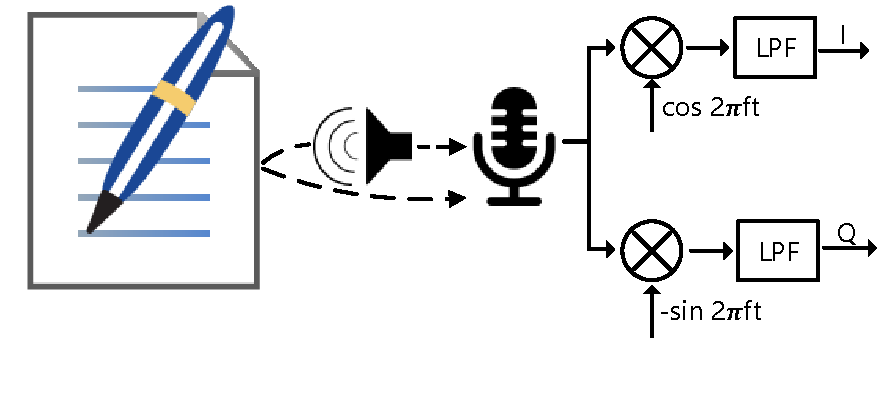
\includegraphics[width=0.7\textwidth]{figure/down-conversion.pdf}
  \bicaption
    {声波信号下转化}
    {Sound signal down conversion}
  \label{fig:sound-signal-down-conversion}
\end{figure}
假设智能手机上的麦克风的采样率设置为48 kHz。由于接收和发射声波的设备在同一智能手机,共享一个时钟频率,因此接收端和发送端之间不存在载频偏移(Carrier Frequency Offset, CFO)。因此,使用图~\ref{fig:sound-signal-down-conversion}所示的传统的相干解调器结构将所接收到的声波信号下转化为基带信号~\cite{tse2005fundamentals}。接收信号被分成两份副本,分别乘以发射信号$-cos2\pi ft$和它的相位偏移信号$-sin2\pi ft$,再经过一个低通滤波器获得同相(In-phase)和正交(Quadrature)分量。

LLAP~\cite{wang2016device}中对信号下转化的过程进行了解释。为了更好得理解数字下转化过程,我们假设一个信号路径$p$的路径长度随时间变化的函数为$d_p\left( t\right)$。来自信号路径$p$可以表示为:
$$
R_{p}\left( t\right) = 2A^{'}_{p}cos \left( 2\pi ft - 2\pi fd_{p}\left( t \right) / c - \theta_{p} \right),
$$
其中,$2A^{'}_{p}$是接收信号的强度,$2\pi fd_{p}\left( t \right)/c$是产生于传播延迟$\tau=d_{p}\left(t\right)/c$的相位间隔,$c$是声音传播速度。初始相位$\theta_p$是硬件延迟和由于反射而发生相位反转的结果。按照图~\ref{fig:sound-signal-down-conversion}中的结构,我们将接收信号乘以$cos\left( 2\pi ft \right)$,得到:
\begin{equation}\nonumber
\begin{aligned}
&2A_{p}^{'}cos \left( 2\pi ft - 2\pi fd_{p}\left( t\right)/c - \theta_{p} \right) \times cos\left( 2\pi ft\right) \\ 
= \quad &A_{p}^{'}\left( cos\left( -2\pi fd_{p}\left( t\right)/c - \theta_{p} \right) + cos\left( 4\pi ft - 2\pi fd_{p}\left( t\right)/c - \theta_{p} \right)  \right).
\end{aligned}
\end{equation}
第二个子项的频率为$2f$,属于高频,可以被低通滤波器所去除。所以我们可以获得基带信号的同相分量(I-component)为:
$$
I_{p}\left( t\right) = A_{p}^{'}cos \left( -2\pi fd_{p}\left( t\right)/c - \theta_{p} \right).
$$
相似地,我们可以获得正交分量(Q-component)为:
$$
Q_{p}\left( t\right)=A_{p}^{'}sin\left( -2\pi fd_{p}\left(t \right)/c - \theta_{p} \right).
$$
结合这两个分量,分别作为复数的实部和虚部,我们可以得到复数形式的基带信号($j^2=-1$):
$$
B_{p}\left( t\right) = A_{p}^{'}e^{-j\left( 2\pi fd_{p}\left( t\right)/c + \theta_{p} \right)}.
$$
因此,在路径$p$上的相位为:
$$
\phi_{p}\left( t\right) = -\left( 2\pi fd_{p}\left( t\right)/c + \theta_{p} \right),
$$当$d_{p}\left(t\right)$变化一个声波波长的长度$\lambda = c/f$时,相位$\phi_{p}\left( t\right)$变化$2\pi$。
\subsection{离散余弦变换}
DCT~\cite{ahmed1974discrete}是一种正交变换,可以用于实现一个维纳滤波器和模式识别中的特征选择。正交变换和逆变换在维纳滤波器中充当重要角色。在模式识别中,DCT可以用于特征选择,对原始数据进行降维,以便于进行分类。一个序列$X(m),m=0,1,\cdots,(M-1)$的DCT可以为定义为:
\begin{equation}
\label{equ:dct}
\begin{aligned}
G_{x}\left( 0\right) &= \frac{\sqrt{2}}{M} \sum_{m=0}^{M-1}X\left( m\right), \\
G_{x}\left( k\right) &= \frac{2}{M} \sum_{m=0}^{M-1}X\left( m\right)cos\frac{\left(2m+1\right)k\pi}{2M}, k=1,2,\cdots,(M-1).
\end{aligned}
\end{equation}
$G_{x}(k)$是第k个DCT系数。值得注意的是,基向量集合$\{ 1/\sqrt{2}, cos((2m+1)k\pi)/(2M) \}$实际上是一组离线切比雪夫多项式。
DCT的逆变换(Inverse Discrete Consine Transform, IDCT)可以被定义为:
\begin{equation}
\label{equ:idct}
X(m) = \frac{1}{\sqrt{2}}G_{x}(0) + \sum_{k=1}^{M-1}G_{x}(k)cos\frac{(2m+1)k\pi}{2M}, m=0,1,\cdots,(M-1). 
\end{equation}
在性能上,DCT好于离散傅里叶变换,接近于最优的Karhunen-Loeve Transform (KLT)。DCT的算法最简单的可以根据上诉的公式进行计算,原文\cite{ahmed1974discrete}中提出了可以使用快速傅里叶变换进行高效计算,之后研究者们提出了一些高效算法~\cite{winograd1978computing,lee1984new,hou1987fast}。

\subsection{卷积神经网络}
\begin{figure}[!htp]
  \centering
  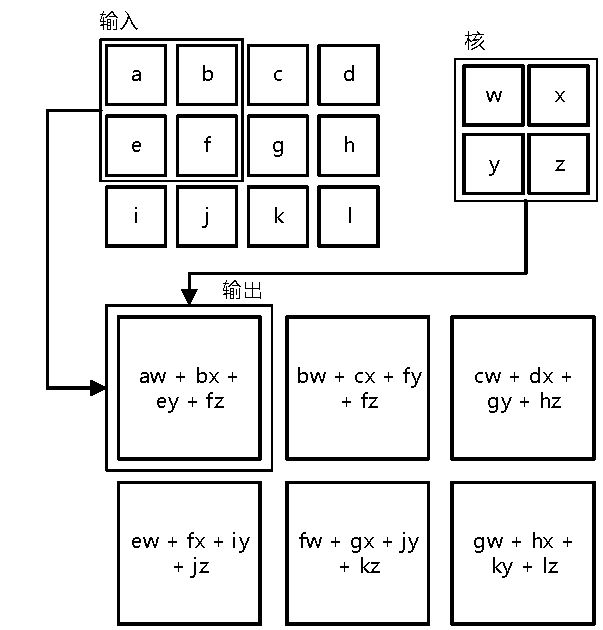
\includegraphics[width=0.6\textwidth]{figure/convolution-process.pdf}
  \bicaption
    {卷积过程}
    {Convolution process}
  \label{fig:convolution-process}
\end{figure}
CNN~\cite{goodfellow2016deep}是一种用于处理网格状数据的特殊ANN,通常包括两类操作:卷积和池化操作,在图像处理领域得到广泛应用。通常被实现为交叉相关函数的卷积操作,在一个输入2维图像(也可以是更高纬的张量)和一个卷积核上生成一个如下的特征图:
$$
S(i,j)=(K\times I)(i,j)=\sum_{m}\sum_{n}I(i+m,j+n)K(m,n),
$$
其中,$I$、$K$、$S$分别是输入图像、卷积核和特征图。图~\ref{fig:convolution-process}演示了一个在二维张量上的卷积运算过程。稀疏交互、参数共享和等变表示是卷积运算中的三个思想,三个思想之间互相影响,是的卷积神经网络只需要较少的模型参数便能实现可靠地特征提取。池化函数使用某个位置的相邻输出的总体统计特征来代替网络在该位置的输出,可对输入进行降维,为神经网络在提供了某种程度平移不变性,常用的池化函数有:最大池化函数、平均池化函数等。


\section{本章小结}
本章是手写签名认证相关技术的分析,首先分别从手写签名认证中的感知技术和手写签名认证中的建模方法两个方面对现有的研究进行了综述,然后分析总结了现有研究存在的问题。基于存在的问题,提出了本文的技术路线,最后介绍了本文中所涉及到的相关理论和技术。

\chapter{基于声波的签名认证方案的关键技术研究}
\section{问题描述与方案设计}
\subsection{问题描述}
本文要解决的问题是利用声波的相位相关信息实现手写签名认证,提出了一种基于声波的一个非侵入式、用户友好、安全、低延迟、准确的在线签名认证方案。其中需要考虑的几个关键的技术问题是音频设备硬件补偿技术技术问题、基于声波的相位相关信息的感知技术问题、基于声波的相位相关信息的特征提取技术问题、以及基于声波特征的建模技术问题。为解决上述问题,本文基于智能手机产品设计实现了一个手写签名认证系统,并在实际场景下部署测试了该系统。

本文列举两个签名认证的例子来描述应用场景,场景一描述我们生活中在银行柜台取款的常见场景便于理解手写签名认证系统的实际作用,场景二则描述了本文所设计系统的可应用场景:
\begin{enumerate}[label=(\arabic*)]
\item \textbf{场景一:}一位叫波波的小伙子去银行取存款,并申明他是这个存款账户的拥有者,然后银行职员要求他前面一边进行一下步操作。根据银行的实际情况,小伙子可能会在一张普通的纸上签字也可能在一个手写平板上签字。接着手写签名认证系统如下运行:首先它从数据库从查询了之前该小伙子留下的参考签名;下一步,它使用设定的算法比较查询签名和参考签名,并计算出查询签名和参考签名之间的相似度。如果系统实时运行的话,银行职员按照签名认证系统的输出结果实行下一步操作。显然,对于基于普通纸张的签名,一个静态的图像将会从纸张上扫描所得,此时签名认证系统为离线签名认证系;然而,基于手写平板的签名,一个额外的时间信息通常被用于提交认证的进度,此时的签名认证系统为在线认证系统。

\begin{figure}[!htp]
  \centering
  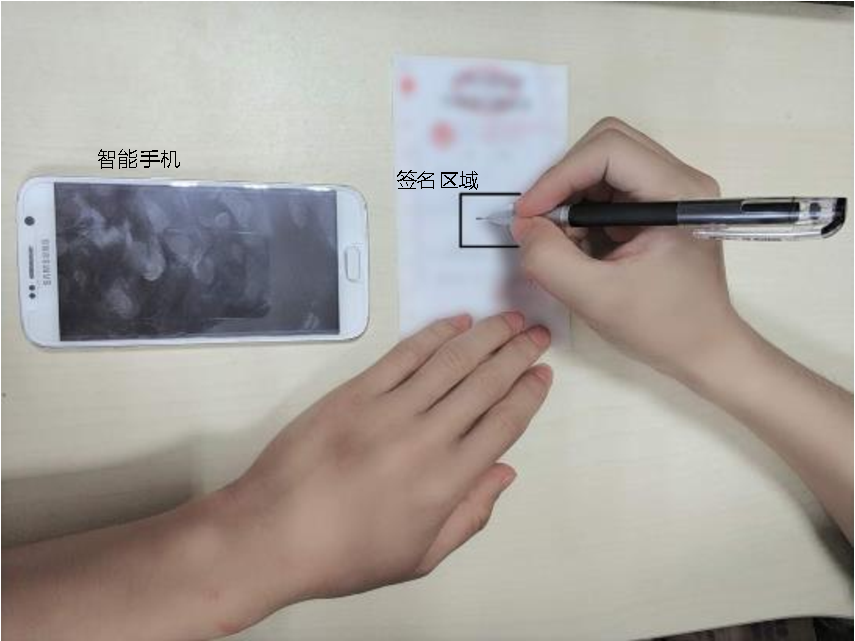
\includegraphics[width=0.6\textwidth]{figure/acoustic-senario.pdf}
  \bicaption
    {签名场景}
    {Senario of signing}
  \label{fig:sign-senario}
\end{figure}

\item  \textbf{场景二:}本文的签名认证方案可以作为一种需要和其他认证方案相结合的辅助认证方案,比如可以和现有的离线签证认证系统或者人工签名认证相集合,最终的系统利用多模的优势而提高签名认证精度。如图~\ref{fig:sign-senario}所示,当一个人在一张现金支票上的签名区域签名时候,他/她将他/她的智能手机放在签名区域旁边记录手和笔在签名动作过程中的模式,该模式将会发送去银行进行识别。纸上的签名将被扫描,作为离线签名认证系统的输入。同时使用不同的权重,两种签名认证方案可以得到融合。值得注意的是,可在支票打印一个二维码,通过二维码可以把智能手机获得签名模式和这个张支票联系起来。
\end{enumerate}

\begin{figure}[!htp]
  \centering
  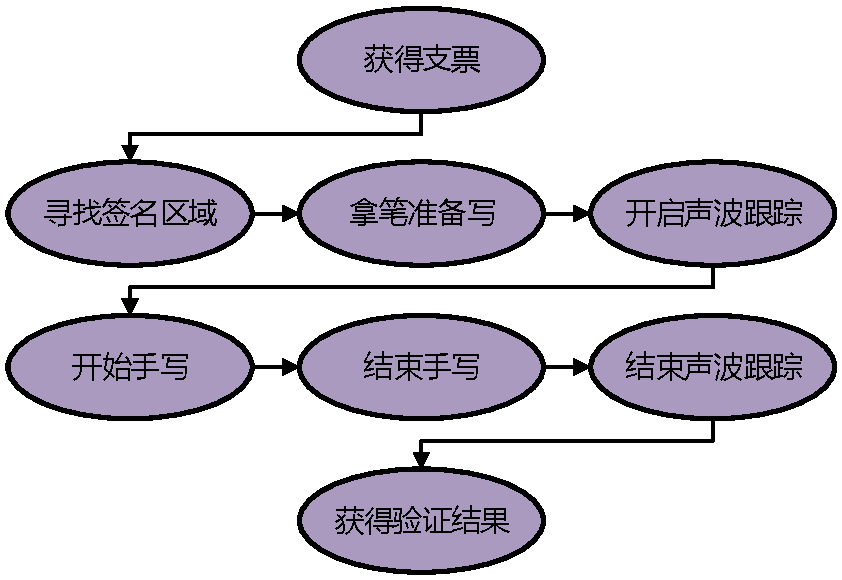
\includegraphics[width=0.6\textwidth]{figure/senario-actions}
  \bicaption
    {场景二签名步骤}
    {Signing steps in Senario 2}
  \label{fig:signing-steps}
\end{figure}

在两个场景中,我们默认认证参考签名已经预先被系统记录下。场景二本文系统所适用的场景,对签证者来说,他/她的操作包括:获取支票、寻找签名区域、拿笔准备写、开启声波跟踪、开始手写、结束手写、结束声波跟踪、获得验证结果。智能手机可以在场景中使用声波跟踪签名过程中手和笔的运动模式。虽然这个注意听起来十分鼓舞人心,但是使用智能手机收发声波跟踪手和笔运动实现在线认证的方案仍然面临着诸多挑战:首先,个人的签名仍然可以被观察和练习,这是目前所有签名认证系统所面临和需要克服的挑战;另外,声波可以被其他恶意的音频接收设备所接收,之后再播放出来实行重放攻击。

\subsection{方案设计}
\begin{figure}[!htp]
  \centering
  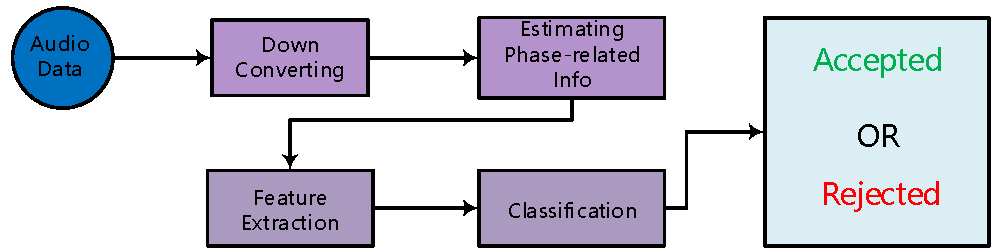
\includegraphics[width=\textwidth]{figure/system-architecture.pdf}
  \bicaption
    {基于声波的手写签名认证方案}
    {Acoustic-based handwritten signature verification method}
  \label{fig:acoustic-hsv-method}
\end{figure}
针对上述问题,本文设计提出了一种基于声波的签名认证方案,如图~\ref{fig:acoustic-hsv-method}所示。该方案主要将声波感知技术引入到手写签名认证的研究中,同时为适应手写签名认证的问题,增加了一系列数据处理技术来完成了方案的设计。该方案共包含四个关键步骤:声波收发、声波相位相关信息采集、特征提取、分类模型。下面依次对每个步骤进行简单介绍。

(1) 声波收发

在发射声波声波之前,首先我们需要设计使用扬声器发射的音频文件,这个音频文件的设计需要考虑用户体验、系统可用性、系统鲁棒性这些特点,而且还需要适配扬声器的硬件特性,进行相应的硬件补偿。


(2) 声波相位相关信息采集

在收到声波反射信号之后,对声波信号进行向下转换从而获得基带信号的两个正交分量。通常在求相位之前,需要对这两个正交分量去直流,然后计算出相位信号,但是在这两个正交信号变化过于多样时,去直流变成异常困难。我们使用了求弦长的方法,估算了相关相关信息(速度和加速度)。其中,除了解决去直流问题,还需要预先对两个正交信号进行去噪。


(3) 特征提取

尽管声波的相关信息是经过降采样的而得,他的数据量仍然较大,不宜直接进行分类。在这个步骤中,对信号进行频域分析,对信号做余弦变换,选择低频信息作为特征,并计算查询签名与参考签名之间的距离矩阵。

(4) 分类模型

本文采用CNN作为二分类的分类模型。模型在调整好参数和使用一些防止过拟合的方法后,使用上一步骤中中距离矩阵作为输入,进行二分类,输出一个范围为0到1的概率值,输出值越大表明输入签名是真是签名的概率越大。

\section{音频设备硬件补偿技术的研究}

本节先介绍原型系统ASSV中的声波信号的设计理念,然后针对设计好的声波信号结合智能手机采取硬件补偿措施。

(1) 声波信号的设计

用于在智能手机上发射声波实际上是使用扬声器播放一个按特定目的设计的音频信号,因此关于声波信号的设计,实际就是关于音频文件中二进制数据序列的设计。为了让麦克风上接收信号可分析,本文设计一种特定的声音让扬声器去发射。在此设计中,本文主要考虑三个方面:用户体验、系统可用性、系统鲁棒性。

\textbf{\textit{(a)} 声波信号设计需要考虑用户体验。}为了让系统提供用户友好型的交互和良好的用户体验,由智能手机发送的声波不应该是可听见的。根据Rodr{\'\i}guez Valiente~\cite{rodriguez2014extended}等人的综叙,当声波的频率高于17 kHz的时候,声音对人便变得不可听。因此,本文生成的声波的频率均大于17 kHz,而且这些声波均可以被商用音频设备(包括本文所用到的智能手机上的扬声器)发射。

\textbf{\textit{(b)} 声波信号设计需要考虑系统可用性。}与LLAP~\cite{wang2016device}中所发射的声波信号相似,为了测量随着传播路径变化的声波信号的相位,ASSV生成声波信号的时候也使用连续波(Continuous Wave, CW)信号:
$$
Acos2\pi ft, 
$$
其中$A$代表信号强度,而$f$代表信号频率。再则,ASSV使用同一个智能手机上的扬声器和麦克风来发射和接收声波,这连个音频设备使用同一个是时钟频率,所以不存在载频偏移问题。如图~\ref{fig:audio-device-smartphone}所示,本文使用的手机上存在两个2个扬声器和2个麦克风。

\begin{figure}
  \centering
  \begin{subfigure}[b]{0.49\textwidth}
    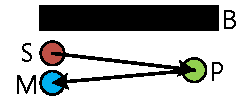
\includegraphics[width=\textwidth]{figure/signal-path-pen-hand-reflected-path}
    \caption{}
    \label{fig:signal-path-pen-hand-reflected-path}
  \end{subfigure}
  \begin{subfigure}[b]{0.49\textwidth}
    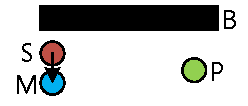
\includegraphics[width=\textwidth]{figure/signal-path-direct-path}
    \caption{}
    \label{fig:signal-path-direct-path}
  \end{subfigure}
  \begin{subfigure}[b]{0.49\textwidth}
    
\includegraphics[width=\textwidth]{figure/signal-path-static-multipath}
    \caption{}
    \label{fig:signal-path-static-multipath}
  \end{subfigure}
  \begin{subfigure}[b]{0.49\textwidth}
    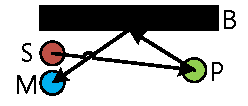
\includegraphics[width=\textwidth]{figure/signal-path-dynamic-multipath}
    \caption{}
    \label{fig:signal-path-dynamic-multipath}
  \end{subfigure}
  \bicaption[信号传播路径]
  {信号传播路径 - (a) 手和笔的反射路径; (b) 直接路径; (c) 静止路径; (d) 动态多径。\textbf{S}, \textbf{M}, \textbf{P}, \textbf{B} 分别代表 扬声器(\textbf{S}peaker), 麦克风(\textbf{M}icrophone), 笔(\textbf{P}en), 障碍物(\textbf{B}lock)。}
  {Signal traveling paths - (a) Hand and pen reflected path; (b) Direct path; (c) Static multipath; (d) Dynamic multipath. \textbf{S}, \textbf{M}, \textbf{P}, \textbf{B} represent \textbf{S}peaker, \textbf{M}icrophone, \textbf{P}en, \textbf{B}lock respectively.}
  \label{fig:signal-travel-paths}
\end{figure}

\textbf{\textit{(c)} 声波信号设计需要系统鲁棒性。}ASSV需要在需要保持鲁棒性,即使多径效应丰富的环境下也需要保持可用的。如图~\ref{fig:signal-travel-paths}所示,我们将声波的传播路径分成4种类型:手和笔的反射路径、直接路径、静止路径和动态多径。
第一种类型,如图~\ref{fig:signal-path-pen-hand-reflected-path}所示,信号从扬声器发出,经过笔和手的反射,传播回到麦克风中。该路径长度随着手写动作的进行而发生变化,实际上,路径是跟踪签名活动中人的行为特征的真正所需要的路径;
第二种类型,本文称这种路径为直接路径。如图~\ref{fig:signal-path-direct-path}所示,信号从直接从扬声器传播到麦克风,没有经任何物体反射。因为直接传播路径所有可能传播路径中最短的一条,所以从直接路径上传播的信号具有最大的能量,换而言之,具有最大的信号波振幅;
第三种类型,本文称这种路径为静止路径。如图~\ref{fig:signal-path-static-multipath}所示,声波仅仅被障碍物反射了一次,图中的障碍物可以是桌子、人的身体等一些在智能附近的禁止可以阻挡声音的障碍物。直接路径和禁止路径传播的声波信号在本文被看作背景信号,手写签名过程中手和笔的运动并不能对背景信号产生丝毫影响;
第四种类型,如图~\ref{fig:signal-path-dynamic-multipath}所示,声波信号从扬声器出发,经过手写过程中的手和笔的反射,再次经过障碍物的反射,最后才传播回到麦克风中。因为障碍物是不确定的,通常是由形状不规则的非结构化的的物体组成,所以经过这种路径传播的声波信号总体上被认为是不稳定和不确定的。

本文使用信号的指数形式来解释最终的接受信号。假设$x_{i}^{'}(t)=A_{i}^{'}e^{-a_{i}^{'}t},x_{j}^{''}(t)=A_{j}^{''}e^{-a_{j}^{''}t},x_{m}^{'''}(t)=A_{m}^{'''}e^{-a_{m}^{'''}t},x_{n}^{''''}(t)=A_{n}^{''''}e^{-a_{n}^{''''}t}$分别表示第一种类型、第二种类型、第三种类型、第四种类型路径中其中一条路径的信号,其中$i,j,m,n$是正整数用于表示“其中一条路径”的意思。假设$X^{'}(t),X^{''}(t),X^{'''}(t),X^{''''}(t)$分别表示四种类型路径上信号的和,$I,J,M,N$分别代表四种类型路径集合中各自的路径数量,我们可以得到:
\begin{eqnarray}
X^{'}(t) &=\quad  \sum_{i=1}^{I}x_{i}^{'}(t)      &=\quad   \sum_{i=1}^{I}A_{i}^{'}e^{-a_{i}^{'}t} \\
X^{''}(t) &=\quad  \sum_{j=1}^{J}x_{j}^{''}(t)     &=\quad  \sum_{j=1}^{J}A_{j}^{''}e^{-a_{j}^{''}t} \\
X^{'''}(t) &=\quad   \sum_{m=1}^{M}x_{m}^{'''}(t)    &=\quad   \sum_{m=1}^{M}A_{m}^{'''}e^{-a_{m}^{'''}t} \\
X^{''''}(t) &=\quad   \sum_{n=1}^{N}x_{n}^{''''}(t)  &=\quad   \sum_{n=1}^{N}A_{n}^{''''}e^{-a_{n}^{''''}t}
\end{eqnarray}
$X(t)$表示麦克风接收的信号,则可以得到:
\begin{equation}\nonumber
\begin{aligned}


\end{aligned}
\end{equation}

总之,第一种传播路径是本文所关心的,第二种和第三种传播路径比较稳定是可以被去除的,而第四种传播路径是我们在设计声波信号着重需要考虑的。通常,结合来自不同频率上的信号的结果可以缓解第四种类型的传播路径最后对结果的影响,这用方法可以被用于提高估计跟踪或者活动识别的精度。

本文选择多个频率高于17 kHz的声波信号组成最后的发射信号。看似所选用的不同的频率的信号越多则越有利于缓解动态多径所产生的影响,但是实际上并不能这样, 不同频率之间存在临频干扰。



\section{基于声波的相位相关信息的感知技术的研究}
\section{基于声波的相位相关信息的特征提取技术的研究}
\section{基于声波特征的建模技术的研究}
\section{本章小结}


\chapter{基于声波的签名认证方案的实验}
\section{实验准备}
\section{硬件补偿评估实验}
\section{精度评估实验}
\section{鲁棒性评估实验}
\section{微基准测试}
\section{经典系统对比实验}
\section{重放攻击实验}

\chapter{基于声波的签名认证方案的系统设计与实现}
\section{系统需求分析}
\section{系统设计与实现}
\section{系统性能评估}
\section{本章小结}

\chapter{总结与展望}
\section{工作总结}
\section{研究展望}
% \section{使用模板}

% \subsection{准备工作}
% \label{sec:requirements}

% 要使用这个模板撰写学位论文,需要在\emph{TeX系统}、\emph{TeX技能}上有所准备。

% \begin{itemize}[noitemsep,topsep=0pt,parsep=0pt,partopsep=0pt]
% 	\item {\TeX}系统:所使用的{\TeX}系统要支持 \XeTeX 引擎,且带有ctex 2.x宏包,以2017年或更新版本的\emph{完整}TeXLive、MacTeX发行版为佳。
% 	\item TeX技能:尽管提供了对模板的必要说明,但这不是一份“ \LaTeX 入门文档”。在使用前请先通读其他入门文档。
% 	\item 针对Windows用户的额外需求:学位论文模本分别使用git和GNUMake进行版本控制和构建,建议从Cygwin\footnote{\url{http://cygwin.com}}安装这两个工具。
% \end{itemize}

% \subsection{模板选项}
% \label{sec:thesisoption}

% sjtuthesis提供了一些常用选项,在thesis.tex在导入sjtuthesis模板类时,可以组合使用。
% 这些选项包括:

% \begin{itemize}[noitemsep,topsep=0pt,parsep=0pt,partopsep=0pt]
% 	\item 学位类型:bachelor(学位)、master(硕士)、doctor(博士),是必选项。
% 	\item 中文字体:fandol(Fandol 开源字体)、windows(Windows 系统下的中文字体)、mac(macOS 系统下的华文字体)、ubuntu(Ubuntu 系统下的文泉驿和文鼎字体)、adobe(Adobe 公司的中文字体)、founder(方正公司的中文字体),默认根据操作系统自动配置。
% 	\item 英文模版:使用english选项启用英文模版。
% 	\item 盲审选项:使用review选项后,论文作者、学号、导师姓名、致谢、发表论文和参与项目将被隐去。
% \end{itemize}

% \subsection{编译模板}
% \label{sec:process}

% 模板默认使用GNUMake构建,GNUMake将调用latemk工具自动完成模板多轮编译:

% \begin{lstlisting}[basicstyle=\small\ttfamily, caption={编译模板}, numbers=none]
% make clean thesis.pdf
% \end{lstlisting}

% 若需要生成包含“原创性声明扫描件”的学位论文文档,请将扫描件保存为statement.pdf,然后调用make生成submit.pdf。

% \begin{lstlisting}[basicstyle=\small\ttfamily, caption={生成用于提交的学位论文}, numbers=none]
% make clean submit.pdf
% \end{lstlisting}

% 编译失败时,可以尝试手动逐次编译,定位故障。

% \begin{lstlisting}[basicstyle=\small\ttfamily, caption={手动逐次编译}, numbers=none]
% xelatex -no-pdf thesis
% biber --debug thesis
% xelatex thesis
% xelatex thesis
% \end{lstlisting}

% \subsection{模板文件布局}
% \label{sec:layout}

% \begin{lstlisting}[basicstyle=\small\ttfamily,caption={模板文件布局},label=layout,float,numbers=none]
% ├── LICENSE
% ├── Makefile
% ├── README.md
% ├── bib
% │   ├── chap1.bib
% │   └── chap2.bib
% ├── bst
% │   └── GBT7714-2005NLang.bst
% ├── figure
% │   ├── chap2
% │   │   ├── sjtulogo.eps
% │   │   ├── sjtulogo.jpg
% │   │   ├── sjtulogo.pdf
% │   │   └── sjtulogo.png
% │   └── sjtubanner.png
% ├── sjtuthesis.cfg
% ├── sjtuthesis.cls
% ├── statement.pdf
% ├── submit.pdf
% ├── tex
% │   ├── abstract.tex
% │   ├── ack.tex
% │   ├── app_cjk.tex
% │   ├── app_eq.tex
% │   ├── app_log.tex
% │   ├── chapter01.tex
% │   ├── chapter02.tex
% │   ├── chapter03.tex
% │   ├── conclusion.tex
% │   ├── id.tex
% │   ├── patents.tex
% │   ├── projects.tex
% │   ├── pub.tex
% │   └── symbol.tex
% └── thesis.tex
% \end{lstlisting}

% 本节介绍学位论文模板中木要文件和目录的功能。

% \subsubsection{格式控制文件}
% \label{sec:format}

% 格式控制文件控制着论文的表现形式,包括sjtuthesis.cfg和sjtuthesis.cls。
% 其中,“cls”控制论文主体格式,“cfg”为配置文件。

% \subsubsection{主控文件thesis.tex}
% \label{sec:thesistex}

% 主控文件thesis.tex的作用就是将你分散在多个文件中的内容“整合”成一篇完整的论文。
% 使用这个模板撰写学位论文时,你的学位论文内容和素材会被“拆散”到各个文件中:
% 譬如各章正文、各个附录、各章参考文献等等。
% 在thesis.tex中通过“include”命令将论文的各个部分包含进来,从而形成一篇结构完成的论文。
% 对模板定制时引入的宏包,建议放在导言区。

% \subsubsection{各章源文件tex}
% \label{sec:thesisbody}

% 这一部分是论文的主体,是以“章”为单位划分的,包括:

% \begin{itemize}[noitemsep,topsep=0pt,parsep=0pt,partopsep=0pt]
% 	\item 中英文摘要(abstract.tex)。前言(frontmatter)的其他部分,中英文封面、原创性声明、授权信息在sjtuthesis.cls中定义,不单独分离为tex文件。
% 不单独弄成文件。
% 	\item 正文(mainmatter)——学位论文正文的各章内容,源文件是chapter\emph{xxx}.tex。
% 	\item 附录(app\emph{xx}.tex)、致谢(ack.tex)、攻读学位论文期间发表的学术论文目录(pub.tex)、个人简历(resume.tex)组成正文后的部分(backmatter)。
% 参考文献列表由bibtex插入,不作为一个单独的文件。
% \end{itemize}

% \subsubsection{图片文件夹figure}
% \label{sec:fig}

% figure文件夹放置了需要插入文档中的图片文件(支持PNG/JPG/PDF/EPS格式的图片),可以在按照章节划分子目录。
% 模板文件中使用\verb|\graphicspath|命令定义了图片存储的顶层目录,在插入图片时,顶层目录名“figure”可省略。

% \subsubsection{参考文献数据库bib}
% \label{sec:bib}

% 目前参考文件数据库目录只存放一个参考文件数据库thesis.bib。
% 关于参考文献引用,可参考第\ref{chap:example}章中的例子。

% 

% %# -*- coding: utf-8-unix -*-
% % !TEX program = xelatex
% % !TEX root = ../thesis.tex
% % !TEX encoding = UTF-8 Unicode
% %%==================================================
% %% chapter02.tex for SJTU Master Thesis
% %% based on CASthesis
% %% modified by wei.jianwen@gmail.com
% %% Encoding: UTF-8
% %%==================================================

% \chapter{{\LaTeX} 排版例子}
% \label{chap:example}

% \section{列表环境}
% \label{sec:list}

% \subsection{无序列表}
% \label{sec:unorderlist}

% 以下是一个无序列表的例子,列表的每个条目单独分段。

% \begin{itemize}
%   \item 这是一个无序列表。
%   \item 这是一个无序列表。
%   \item 这是一个无序列表。
% \end{itemize}

% 使用\verb+itemize*+环境可以创建行内无序列表。
% \begin{itemize*}
%   \item 这是一个无序列表。
%   \item 这是一个无序列表。
%   \item 这是一个无序列表。
% \end{itemize*}
% 行内无序列表条目不单独分段,所有内容直接插入在原文的段落中。

% \subsection{有序列表}
% \label{sec:orderlist}

% 使用环境\verb+enumerate+和\verb+enumerate*+创建有序列表,
% 使用方法无序列表类似。

% \begin{enumerate}
%   \item 这是一个有序列表。
%   \item 这是一个有序列表。
%   \item 这是一个有序列表。
% \end{enumerate}

% 使用\verb+enumerate*+环境可以创建行内有序列表。
% \begin{enumerate*}
%   \item 这是一个默认有序列表。
%   \item 这是一个默认有序列表。
%   \item 这是一个默认有序列表。
% \end{enumerate*}
% 行内有序列表条目不单独分段,所有内容直接插入在原文的段落中。

% \subsection{描述型列表}

% 使用环境\verb+description+可创建带有主题词的列表,条目语法是\verb+\item[主题] 内容+。
% \begin{description}
%     \item[主题一] 详细内容
%     \item[主题二] 详细内容
%     \item[主题三] 详细内容 \ldots
% \end{description}

% \subsection{自定义列表样式}

% 可以使用\verb+label+参数控制列表的样式,
% 详细可以参考WikiBooks\footnote{\url{https://en.wikibooks.org/wiki/LaTeX/List_Structures\#Customizing_lists}}。
% 比如一个自定义样式的行内有序列表
% \begin{enumerate*}[label=\itshape\alph*)\upshape]
%   \item 这是一个自定义样式有序列表。
%   \item 这是一个自定义样式有序列表。
%   \item 这是一个自定义样式有序列表。
% \end{enumerate*}

% \section{数学排版}
% \label{sec:matheq}

% \subsection{公式排版}
% \label{sec:eqformat}

% 这里有举一个长公式排版的例子,来自\href{http://www.tex.ac.uk/tex-archive/info/math/voss/mathmode/Mathmode.pdf}{《Math mode》}:

% \begin {multline}
%   \frac {1}{2}\Delta (f_{ij}f^{ij})=
%   2\left (\sum _{i<j}\chi _{ij}(\sigma _{i}-
%     \sigma _{j}) ^{2}+ f^{ij}\nabla _{j}\nabla _{i}(\Delta f)+\right .\\
%   \left .+\nabla _{k}f_{ij}\nabla ^{k}f^{ij}+
%     f^{ij}f^{k}\left [2\nabla _{i}R_{jk}-
%       \nabla _{k}R_{ij}\right ]\vphantom {\sum _{i<j}}\right )
% \end{multline}

% \subsection{SI单位}

% 使用\verb+siunitx+宏包可以方便地输入SI单位制单位,例如\verb+\SI{5}{\um}+可以得到\SI{5}{\um}。

% \subsubsection{一个四级标题}
% \label{sec:depth4}

% 这是全文唯一的一个四级标题。在这部分中将演示了mathtools宏包中可伸长符号(箭头、等号的例子)的例子。

% \begin{displaymath}
%     A \xleftarrow[n=0]{} B \xrightarrow[LongLongLongLong]{n>0} C
% \end{displaymath}

% \begin{eqnarray}
%   f(x) & \xleftrightarrow[]{A=B}  & B \\
%   & \xleftharpoondown[below]{above} & B \nonumber \\
%   & \xLeftrightarrow[below]{above} & B
% \end{eqnarray}

% 又如:

% \begin{align}
%   \label{eq:none}
%   & I(X_3;X_4)-I(X_3;X_4\mid{}X_1)-I(X_3;X_4\mid{}X_2) \nonumber \\
%   = & [I(X_3;X_4)-I(X_3;X_4\mid{}X_1)]-I(X_3;X_4\mid{}\tilde{X}_2) \\
%   = & I(X_1;X_3;X_4)-I(X_3;X_4\mid{}\tilde{X}_2)
% \end{align}

% \subsection{定理环境}

% 模板中定义了丰富的定理环境
% algo(算法),thm(定理),lem(引理),prop(命题),cor(推论),defn(定义),conj(猜想),exmp(例),rem(注),case(情形),
% bthm(断言定理),blem(断言引理),bprop(断言命题),bcor(断言推论)。
% amsmath还提供了一个proof(证明)的环境。
% 这里举一个“定理”和“证明”的例子。
% \begin{thm}[留数定理]
% \label{thm:res}
%   假设$U$是复平面上的一个单连通开子集,$a_1,\ldots,a_n$是复平面上有限个点,$f$是定义在$U\backslash \{a_1,\ldots,a_n\}$上的全纯函数,
%   如果$\gamma$是一条把$a_1,\ldots,a_n$包围起来的可求长曲线,但不经过任何一个$a_k$,并且其起点与终点重合,那么:

%   \begin{equation}
%     \label{eq:res}
%     \ointop_{\gamma}f(z)\,\mathrm{d}z = 2\uppi\mathbf{i}\sum^n_{k=1}\mathrm{I}(\gamma,a_k)\mathrm{Res}(f,a_k)
%   \end{equation}

%   如果$\gamma$是若尔当曲线,那么$\mathrm{I}(\gamma, a_k)=1$,因此:

%   \begin{equation}
%     \label{eq:resthm}
%     \ointop_{\gamma}f(z)\,\mathrm{d}z = 2\uppi\mathbf{i}\sum^n_{k=1}\mathrm{Res}(f,a_k)
%   \end{equation}

%       % \oint_\gamma f(z)\, dz = 2\pi i \sum_{k=1}^n \mathrm{Res}(f, a_k ).

%   在这里,$\mathrm{Res}(f, a_k)$表示$f$在点$a_k$的留数,$\mathrm{I}(\gamma,a_k)$表示$\gamma$关于点$a_k$的卷绕数。
%   卷绕数是一个整数,它描述了曲线$\gamma$绕过点$a_k$的次数。如果$\gamma$依逆时针方向绕着$a_k$移动,卷绕数就是一个正数,
%   如果$\gamma$根本不绕过$a_k$,卷绕数就是零。

%   定理\ref{thm:res}的证明。

%   \begin{proof}
%     首先,由……

%     其次,……

%     所以……
%   \end{proof}
% \end{thm}

% 上面的公式例子中,有一些细节希望大家注意。微分号d应该使用“直立体”也就是用mathrm包围起来。
% 并且,微分号和被积函数之间应该有一段小间隔,可以插入\verb+\,+得到。
% 斜体的$d$通常只作为一般变量。
% i,j作为虚数单位时,也应该使用“直立体”为了明显,还加上了粗体,例如\verb+\mathbf{i}+。斜体$i,j$通常用作表示“序号”。
% 其他字母在表示常量时,也推荐使用“直立体”譬如,圆周率$\uppi$(需要upgreek宏包),自然对数的底$\mathrm{e}$。
% 不过,我个人觉得斜体的$e$和$\pi$很潇洒,在不至于引起混淆的情况下,我也用这两个字母的斜体表示对应的常量。


% \section{向文档中插入图像}
% \label{sec:insertimage}

% \subsection{支持的图片格式}
% \label{sec:imageformat}

% \XeTeX 可以很方便地插入PDF、PNG、JPG格式的图片。

% 插入PNG/JPG的例子如\ref{fig:SRR}所示。
% 这两个水平并列放置的图共享一个“图标题”(table caption),没有各自的小标题。

% \begin{figure}[!htp]
%   \centering
%   \includegraphics[width=4cm]{example/sjtulogo.png}
%   \hspace{1cm}
%   \includegraphics[width=4cm]{example/sjtulogo.jpg}
%   \bicaption[这里将出现在插图索引中]
%     {中文题图}
%     {English caption}
%   \label{fig:SRR}
% \end{figure}

% 这里还有插入EPS图像和PDF图像的例子,如图\ref{fig:epspdf:a}和图\ref{fig:epspdf:b}。这里将EPS和PDF图片作为子图插入,每个子图有自己的小标题。子图标题使用subcaption宏包添加。

% \begin{figure}[!htp]
%   \centering
%   \subcaptionbox{EPS 图像\label{fig:epspdf:a}}[3cm] %标题的长度,超过则会换行,如下一个小图。
%     {\includegraphics[height=2.5cm]{example/sjtulogo.eps}}
%   \hspace{4em}
%   \subcaptionbox{PDF 图像,注意这个图略矮些。如果标题很长的话,它会自动换行\label{fig:epspdf:b}}
%     {\includegraphics[height=2cm]{sjtulogo.pdf}}
%   \bicaption{插入eps和pdf的例子(使用 subcaptionbox 方式)}{An EPS and PDF demo with subcaptionbox}
%   \label{fig:pdfeps-subcaptionbox}
% \end{figure}

% \begin{figure}[!htp]
%   \centering
%   \begin{subfigure}{2.5cm}
%     \centering
%     \includegraphics[height=2.5cm]{example/sjtulogo.eps}
%     \caption{EPS 图像}
%   \end{subfigure}
%   \hspace{4em}
%   \begin{subfigure}{0.4\textwidth}
%     \centering
%     \includegraphics[height=2cm]{sjtulogo.pdf}
%     \caption{PDF 图像,注意这个图略矮些。subfigure中同一行的子图在顶端对齐。}
%   \end{subfigure}
%   \bicaption{插入eps和pdf的例子(使用 subfigure 方式)}{An EPS and PDF demo with subfigure}
%   \label{fig:pdfeps-subfigure}
% \end{figure}

% 更多关于 \LaTeX 插图的例子可以参考\href{http://www.cs.duke.edu/junhu/Graphics3.pdf}{《\LaTeX 插图指南》}。

% \subsection{长标题的换行}
% \label{sec:longcaption}

% 图\ref{fig:longcaptionbad}和图\ref{fig:longcaptiongood}都有比较长图标题,通过对比发现,图\ref{fig:longcaptiongood}的换行效果更好一些。
% 其中使用了minipage环境来限制整个浮动体的宽度。

% \begin{figure}[!htp]
%   \centering
%   \includegraphics[width=4cm]{sjtubadge.pdf}
%   \bicaption[这里将出现在插图索引]
%     {上海交通大学是我国历史最悠久的高等学府之一,是教育部直属、教育部与上海市共建的全国重点大学.}
%     {Where there is a will, there is a way.}
%  \label{fig:longcaptionbad}
% \end{figure}

% \begin{figure}[!htbp]
%   \centering
%   \begin{minipage}[b]{0.6\textwidth}
%     \centering
%     \includegraphics[width=4cm]{sjtubadge.pdf}
%     \bicaption[出现在插图索引中]
%       {上海交通大学是我国历史最悠久的高等学府之一,是教育部直属、教育部与上海市共建的全国重点大学.}
%       {Where there is a will, there is a way.}
%     \label{fig:longcaptiongood}
%   \end{minipage}
% \end{figure}

% \subsection{添加图注}

% 当插图中组成部件由数字或字母等编号表示时,可在插图下方添加图注进行说明,如图\ref{fig:cn_100t}所示。

% \begin{figure}[!htp]
%   \centering
%   \includegraphics[width=0.3\textwidth]{example/cn_100t.png}\
%   \begin{center}
%     \small\kaishu 1.立柱 2.提升释放机构 3.标准冲击加速度计 \\ 4.导轨 5.重锤 6.被校力传感器 7.底座
%   \end{center}
%   \vspace{-1em}
%   \bicaption[出现在插图索引中]
%     {示例图片来源于\parencite{he1999}}
%     {Stay hungry, stay foolish.}
%  \label{fig:cn_100t}
% \end{figure}

% \subsection{绘制流程图}

% 图\ref{fig:flow_chart}是一张流程图示意。使用tikz环境,搭配四种预定义节点(\verb+startstop+、\verb+process+、\verb+decision+和\verb+io+),可以容易地绘制出流程图。
% \begin{figure}[!htp]
%     \centering
%     \resizebox{6cm}{!}{\input{figure/example/flow_chart.tex}}
%     \bicaption{绘制流程图效果}{Flow chart}
%     \label{fig:flow_chart}
% \end{figure}

% \clearpage

% \section{表格}
% \label{sec:tab}

% 这一节给出的是一些表格的例子,如表\ref{tab:firstone}所示。

% \begin{table}[!hpb]
%   \centering
%   \bicaption[指向一个表格的表目录索引]
%     {一个颇为标准的三线表格\footnotemark[1]}
%     {A Table}
%   \label{tab:firstone}
%   \begin{tabular}{@{}llr@{}} \toprule
%     \multicolumn{2}{c}{Item} \\ \cmidrule(r){1-2}
%     Animal & Description & Price (\$)\\ \midrule
%     Gnat & per gram & 13.65 \\
%     & each & 0.01 \\
%     Gnu & stuffed & 92.50 \\
%     Emu & stuffed & 33.33 \\
%     Armadillo & frozen & 8.99 \\ \bottomrule
%   \end{tabular}
% \end{table}
% \footnotetext[1]{这个例子来自\href{http://www.ctan.org/tex-archive/macros/latex/contrib/booktabs/booktabs.pdf}{《Publication quality tables in LATEX》}(booktabs宏包的文档)。这也是一个在表格中使用脚注的例子,请留意与threeparttable实现的效果有何不同。}

% 下面一个是一个更复杂的表格,用threeparttable实现带有脚注的表格,如表\ref{tab:footnote}。

% \begin{table}[!htpb]
%   \bicaption[出现在表目录的标题]
%     {一个带有脚注的表格的例子}
%     {A Table with footnotes}
%   \label{tab:footnote}
%   \centering
%   \begin{threeparttable}[b]
%      \begin{tabular}{ccd{4}cccc}
%       \toprule
%       \multirow{2}{6mm}{total}&\multicolumn{2}{c}{20\tnote{1}} & \multicolumn{2}{c}{40} &  \multicolumn{2}{c}{60}\\
%       \cmidrule(lr){2-3}\cmidrule(lr){4-5}\cmidrule(lr){6-7}
%       &www & \multicolumn{1}{c}{k} & www & k & www & k \\ % 使用说明符 d 的列会自动进入数学模式,使用 \multicolumn 对文字表头做特殊处理
%       \midrule
%       &$\underset{(2.12)}{4.22}$ & 120.0140\tnote{2} & 333.15 & 0.0411 & 444.99 & 0.1387 \\
%       &168.6123 & 10.86 & 255.37 & 0.0353 & 376.14 & 0.1058 \\
%       &6.761    & 0.007 & 235.37 & 0.0267 & 348.66 & 0.1010 \\
%       \bottomrule
%     \end{tabular}
%     \begin{tablenotes}
%     \item [1] the first note.% or \item [a]
%     \item [2] the second note.% or \item [b]
%     \end{tablenotes}
%   \end{threeparttable}
% \end{table}

% \section{参考文献管理}

%  \LaTeX 具有将参考文献内容和表现形式分开管理的能力,涉及三个要素:参考文献数据库、参考文献引用格式、在正文中引用参考文献。
% 这样的流程需要多次编译:

% \begin{enumerate}[noitemsep,topsep=0pt,parsep=0pt,partopsep=0pt]
% 	\item 用户将论文中需要引用的参考文献条目,录入纯文本数据库文件(bib文件)。
% 	\item 调用xelatex对论文模板做第一次编译,扫描文中引用的参考文献,生成参考文献入口文件(aux)文件。
% 	\item 调用bibtex,以参考文献格式和入口文件为输入,生成格式化以后的参考文献条目文件(bib)。
% 	\item 再次调用xelatex编译模板,将格式化以后的参考文献条目插入正文。
% \end{enumerate}

% 参考文献数据库(thesis.bib)的条目,可以从Google Scholar搜索引擎\footnote{\url{https://scholar.google.com}}、CiteSeerX搜索引擎\footnote{\url{http://citeseerx.ist.psu.edu}}中查找,文献管理软件Papers\footnote{\url{http://papersapp.com}}、Mendeley\footnote{\url{http://www.mendeley.com}}、JabRef\footnote{\url{http://jabref.sourceforge.net}}也能够输出条目信息。

% 下面是在Google Scholar上搜索到的一条文献信息,格式是纯文本:

% \begin{lstlisting}[caption={从Google Scholar找到的参考文献条目}, label=googlescholar, escapeinside="", numbers=none]
%     @phdthesis{"白2008信用风险传染模型和信用衍生品的定价",
%       title={"信用风险传染模型和信用衍生品的定价"},
%       author={"白云芬"},
%       year={2008},
%       school={"上海交通大学"}
%     }
% \end{lstlisting}

% 推荐修改后在bib文件中的内容为:

% \begin{lstlisting}[caption={修改后的参考文献条目}, label=itemok, escapeinside="", numbers=none]
%   @phdthesis{bai2008,
%     title={"信用风险传染模型和信用衍生品的定价"},
%     author={"白云芬"},
%     date={2008},
%     address={"上海"},
%     school={"上海交通大学"}
%   }
% \end{lstlisting}

% 按照教务处的要求,参考文献外观应符合国标GBT7714的要求\footnote{\url{http://www.cces.net.cn/guild/sites/tmxb/Files/19798_2.pdf}}。
% 在模板中,表现形式的控制逻辑通过biblatex-gb7714-2015包实现\footnote{\url{https://www.ctan.org/pkg/biblatex-gb7714-2015}},基于{Bib\LaTeX}管理文献。在目前的多数TeX发行版中,可能都没有默认包含biblatex-gb7714-2015,需要手动安装。

% 正文中引用参考文献时,用\verb+\cite{key1,key2,key3...}+可以产生“上标引用的参考文献”,
% 如\cite{Meta_CN,chen2007act,DPMG}。
% 使用\verb+\parencite{key1,key2,key3...}+则可以产生水平引用的参考文献,例如\parencite{JohnD,zhubajie,IEEE-1363}。
% 请看下面的例子,将会穿插使用水平的和上标的参考文献:关于书的\parencite{Meta_CN,JohnD,IEEE-1363},关于期刊的\cite{chen2007act,chen2007ewi},
% 会议论文\parencite{DPMG,kocher99,cnproceed},
% 硕士学位论文\parencite{zhubajie,metamori2004},博士学位论文\cite{shaheshang,FistSystem01,bai2008},标准文件\parencite{IEEE-1363},技术报告\cite{NPB2},电子文献\parencite{xiaoyu2001, CHRISTINE1998},用户手册\parencite{RManual}。

% 总结一些注意事项:
% \begin{itemize}
% \item 参考文献只有在正文中被引用了,才会在最后的参考文献列表中出现;
% \item 参考文献“数据库文件”bib是纯文本文件,请使用UTF-8编码,不要使用GBK编码;
% \item 参考文献条目中默认通过date域输入时间。兼容使用year域时会产生编译warning,可忽略。
% \end{itemize}

% \section{用listings插入源代码}

% 原先ctexbook文档类和listings宏包配合使用时,代码在换页时会出现莫名其妙的错误,后来经高人指点,顺利解决了。
% 感兴趣的话,可以看看\href{http://bbs.ctex.org/viewthread.php?tid=53451}{这里}。
% 这里给使用listings宏包插入源代码的例子,这里是一段C代码。
% 另外,listings宏包真可谓博大精深,可以实现各种复杂、漂亮的效果,想要进一步学习的同学,可以参考
% \href{http://mirror.ctan.org/macros/latex/contrib/listings/listings.pdf}{listings宏包手册}。

% \begin{lstlisting}[language={C}, caption={一段C源代码}]
% #include <stdio.h>
% #include <unistd.h>
% #include <sys/types.h>
% #include <sys/wait.h>

% int main() {
%   pid_t pid;

%   switch ((pid = fork())) {
%   case -1:
%     printf("fork failed\n");
%     break;
%   case 0:
%     /* child calls exec */
%     execl("/bin/ls", "ls", "-l", (char*)0);
%     printf("execl failed\n");
%     break;
%   default:
%     /* parent uses wait to suspend execution until child finishes */
%     wait((int*)0);
%     printf("is completed\n");
%     break;
%   }

%   return 0;
% }
% \end{lstlisting}

% \section{用algorithm和algorithmicx宏包插入算法描述}

% algorithmicx 比 algorithmic 增加了一些命令。
% 示例如算法\ref{algo:sum_100}和算法\ref{algo:merge_sort},
% 后者的代码来自\href{http://hustsxh.is-programmer.com/posts/38801.html}{xhSong的博客}。
% algorithmicx的详细使用方法见\href{http://mirror.hust.edu.cn/CTAN/macros/latex/contrib/algorithmicx/algorithmicx.pdf}{官方README}。
% 使用算法宏包时,算法出现的位置很多时候不按照tex文件里的书写顺序,
% 需要强制定位时可以使用\verb+\begin{algorithm}[H]+
% \footnote{http://tex.stackexchange.com/questions/165021/fixing-the-location-of-the-appearance-in-algorithmicx-environment}

% 这是写在算法\ref{algo:sum_100}前面的一段话,在生成的文件里它会出现在算法\ref{algo:sum_100}前面。

% \begin{algorithm}
% % \begin{algorithm}[H] % 强制定位
% \caption{求100以内的整数和}
% \label{algo:sum_100}
% \begin{algorithmic}[1] %每行显示行号
% \Ensure 100以内的整数和 % 输出
% \State $sum \gets 0$
% \For{$i = 0 \to 100$}
%     \State $sum \gets sum + i$
%   \EndFor
% \end{algorithmic}
% \end{algorithm}

% 这是写在两个算法中间的一段话,当算法\ref{algo:sum_100}不使用\verb+\begin{algorithm}[H]+时它也会出现在算法\ref{algo:sum_100}前面。

% 对于很长的算法,单一的算法块\verb+\begin{algorithm}...\end{algorithm}+是不能自动跨页的
% \footnote{http://tex.stackexchange.com/questions/70733/latex-algorithm-not-display-under-correct-section},
% 会出现的情况有:

% \begin{itemize}
%   \item 该页放不下当前的算法,留下大片空白,算法在下一页显示
%   \item 单一页面放不下当前的算法,显示时超过页码的位置直到超出整个页面范围
% \end{itemize}

% 解决方法有:

% \begin{itemize}
%   \item (推荐)使用\verb+algstore{algname}+和\verb+algrestore{algname}+来讲算法分为两个部分\footnote{http://tex.stackexchange.com/questions/29816/algorithm-over-2-pages},如算法\ref{algo:merge_sort}。
%   \item 人工拆分算法为多个小的部分。
% \end{itemize}

% \begin{algorithm}
% % \begin{algorithm}[H] % 强制定位
% \caption{用归并排序求逆序数}
% \label{algo:merge_sort}
% \begin{algorithmic}[1] %每行显示行号
% \Require $Array$数组,$n$数组大小 % 输入
% \Ensure 逆序数 % 输出
% \Function {MergerSort}{$Array, left, right$}
%   \State $result \gets 0$
%   \If {$left < right$}
%     \State $middle \gets (left + right) / 2$
%     \State $result \gets result +$ \Call{MergerSort}{$Array, left, middle$}
%     \State $result \gets result +$ \Call{MergerSort}{$Array, middle, right$}
%     \State $result \gets result +$ \Call{Merger}{$Array,left,middle,right$}
%   \EndIf
%   \State \Return{$result$}
% \EndFunction
% \State %空一行
% \Function{Merger}{$Array, left, middle, right$}
%   \State $i\gets left$
%   \State $j\gets middle$
%   \State $k\gets 0$
%   \State $result \gets 0$
%   \While{$i<middle$ \textbf{and} $j<right$}
%     \If{$Array[i]<Array[j]$}
%       \State $B[k++]\gets Array[i++]$
%     \Else
%       \State $B[k++] \gets Array[j++]$
%       \State $result \gets result + (middle - i)$
%     \EndIf
%   \EndWhile
%   \algstore{MergeSort}
% \end{algorithmic}
% \end{algorithm}

% \begin{algorithm}
% \begin{algorithmic}[1]
%   \algrestore{MergeSort}
%   \While{$i<middle$}
%     \State $B[k++] \gets Array[i++]$
%   \EndWhile
%   \While{$j<right$}
%     \State $B[k++] \gets Array[j++]$
%   \EndWhile
%   \For{$i = 0 \to k-1$}
%     \State $Array[left + i] \gets B[i]$
%   \EndFor
%   \State \Return{$result$}
% \EndFunction
% \end{algorithmic}
% \end{algorithm}

% 这是写在算法\ref{algo:merge_sort}后面的一段话,
% 但是当算法\ref{algo:merge_sort}不使用\verb+\begin{algorithm}[H]+时它会出现在算法\ref{algo:merge_sort}
% 甚至算法\ref{algo:sum_100}前面。

% 对于算法的索引要注意\verb+\caption+和\verb+\label+的位置,
% 必须是先\verb+\caption+再\verb+\label+\footnote{http://tex.stackexchange.com/questions/65993/algorithm-numbering},
% 否则会出现\verb+\ref{algo:sum_100}+生成的编号跟对应算法上显示不一致的问题。

% 根据Werner的回答\footnote{http://tex.stackexchange.com/questions/53357/switch-cases-in-algorithmic}
% 增加了\verb+Switch+和\verb+Case+的支持,见算法\ref{algo:switch_example}。

% \begin{algorithm}
% \caption{Switch示例}
% \label{algo:switch_example}
% \begin{algorithmic}[1]
%   \Switch{$s$}
%     \Case{$a$}
%       \Assert{0}
%     \EndCase
%     \Case{$b$}
%       \Assert{1}
%     \EndCase
%     \Default
%       \Assert{2}
%     \EndDefault
%   \EndSwitch
% \end{algorithmic}
% \end{algorithm}

%\include{tex/faq}
%\include{tex/summary}

%\appendix % 使用英文字母对附录编号

% 附录内容,本科学位论文可以用翻译的文献替代。
%\include{tex/app_setup}
%\include{tex/app_eq}
%\include{tex/app_cjk}
%\include{tex/app_log}

\backmatter % 文后无编号部分 

% 参考资料
\printbibliography[heading=bibintoc]

% 致谢、发表论文、申请专利、参与项目、简历
% 用于盲审的论文需隐去致谢、发表论文、申请专利、参与的项目
\makeatletter

% "研究生学位论文送盲审印刷格式的统一要求"
% http://www.gs.sjtu.edu.cn/inform/3/2015/20151120_123928_738.htm

% 盲审删去删去致谢页
\ifsjtu@review\relax\else
  %# -*- coding: utf-8-unix -*-
% !TEX program = xelatex
% !TEX root = ../thesis.tex
% !TEX encoding = UTF-8 Unicode
\begin{thanks}
岁月如梭,一眨眼,两年半时间已然过去,仿佛昨天我刚入学,进入却已经开始要毕业走上社会。在此,我想感谢在这珍贵的研究生生涯帮助过我,给我力量的老师、同学和亲人们。是你们的支持和鼓励,让我的这两年半的路途走得如此顺畅。

感谢我的导师王东老师。还记得,第一次见王老师是在夏令营的时候,王老师激情四射的演讲风格深深地吸引了我和我的同学。进入实验室后,除了生活上的关心,王老师给了很多科研上的指导,不断督促我的科研进展,遇到困难时召集师兄们帮我一起解决困难和指引正确的方向,给予适当的鼓励。王老师,除了是科研上的导师外,还是一位人生导师,严谨的处事风格和友善的待人风格对我启发颇深。王老师,是我科研上的导师,也是我饭桌上的朋友。

感谢两位博士师兄——赵润和张谦,两位师兄以丰富的学识征服了我。在组会上,经常能给我的研究给出宝贵的建议,以自己深刻见解指引我走向正确的方向。和两位师兄的接触,也让我虽然不读博也能了解博士的生活,增长了我的见识。赵润师兄是个二次元,也是我附近最年长的师兄,可以给我展示一个不一样的世界,在生活给我提供了很多经验之谈,让我受益匪浅。张谦师兄是个暖男,很友善,易于相处,总能细心解答我的疑问。另外,感谢李冬师兄在我初进实验室时,给予热心的生活和科研上的帮助。和三位师兄一起的澳门之行,让我至今记忆犹新。

感谢实验室和我同届的邓毓峰、陈渤、黄安娜、徐华韬、朱艳、江浩、黄思和秦培杰,是你们在我狭小的研究生圈子里,提供了一个良好健康的生活和学习氛围。实验室同学认真学习和放开玩耍的样子都很酷。我会好好珍惜你们在一起度过的时光,包括舟山春游、物联网志愿者、组会、饭局等,一起玩耍大大增进了我们之间的情谊。

感谢我的父母和家人,是你们的支持使我顺利完成学业,你们的支持和关怀不仅给与我心灵上的蕴藉,还成为我坚持奋斗的不竭动力,是你们让我更加乐观地面对生活中的一切,感谢你们对我如此无私的付出,我将用一生去回报。

再次感谢所有给予我关心、支持和帮助的老师、同学、亲人们!未来的生活和工作中我会继续努力,争取创造更大的成就。

\end{thanks}
         % 致谢
\fi

\ifsjtu@bachelor
  % 学士学位论文要求在最后有一个英文大摘要,单独编页码
  \include{tex/end_english_abstract}
\else
  % 盲审论文中,发表学术论文及参与科研情况等仅以第几作者注明即可,不要出现作者或他人姓名
  \ifsjtu@review\relax
    %# -*- coding: utf-8-unix -*-
% !TEX program = xelatex
% !TEX root = ../thesis.tex
% !TEX encoding = UTF-8 Unicode

\begin{publications}{99}
    \item\textsc{第一作者}. {ASSV: handwritten signature verification using acoustic signals
}, 2019.
    \item\textsc{第一作者}. {TTBA: An RFID-based Tracking System for Two Basic Actions in Free-Weight Exercises
}, 2018.
\end{publications}

    %# -*- coding: utf-8-unix -*-
% !TEX program = xelatex
% !TEX root = ../thesis.tex
% !TEX encoding = UTF-8 Unicode

\begin{projects}{99}
    \item 上海市科学技术委员会平台建设项目%(2007年6月--2008年5月)
    \item 上海市经济和信息化委员会、上海市人力资源和社会保障局上海市高技能人才培养基地资助项目%(2005年5月--2005年8月)
\end{projects}
  
  \else
    %# -*- coding: utf-8-unix -*-
% !TEX program = xelatex
% !TEX root = ../thesis.tex
% !TEX encoding = UTF-8 Unicode
%%==================================================
%% pub.tex for SJTUThesis
%% Encoding: UTF-8
%%==================================================

\begin{publications}{99}
    \item\textsc{Feng Ding, Qian Zhang, Run Zhao and Dong Wang}. TTBA: An RFID-based Tracking System for Two Basic Actions in Free-Weight Exercises[C]//Proceedings of the 14th ACM International Symposium on QoS and Security for Wireless and Mobile Networks. ACM, 2018: 7-14.
    \item\textsc{Dong Li, Feng Ding, Qian Zhang, Run Zhao, Jinshi Zhang and Dong Wang}. TagController: A Universal Wireless and Battery-free Remote Controller using Passive RFID Tags[C]//Proceedings of the 14th EAI International Conference on Mobile and Ubiquitous Systems: Computing, Networking and Services. ACM, 2017: 166-175.
\end{publications}
       % 发表论文
    %# -*- coding: utf-8-unix -*-
% !TEX program = xelatex
% !TEX root = ../thesis.tex
% !TEX encoding = UTF-8 Unicode
%%==================================================
%% projects.tex for SJTUThesis
%% Encoding: UTF-8
%%==================================================

\begin{projects}{99}
    \item 上海市科学技术委员会平台建设项目“上海射频识别工程技术研究中心”
    \item 上海市经济和信息化委员会、上海市人力资源和社会保障局上海市高技能人才培养基地资助项目“上海市物联网技术高技能人才培养基地实训设施设备(RFID应用)资助项目”
\end{projects}
  % 参与的项目
    % \include{tex/patents}   % 申请专利
    \include{tex/resume}    % 个人简历
  \fi
\fi

\makeatother

\end{document}
